%% LaTeX2e class for student theses
%% sections/evaluation.tex
%% 
%% Karlsruhe Institute of Technology
%% Institute for Program Structures and Data Organization
%% Chair for Software Design and Quality (SDQ)
%%
%% Dr.-Ing. Erik Burger
%% burger@kit.edu
%%
%% Version 1.1, 2014-11-21

\chapter{Validierung}
\label{ch:validierung}
In diesem Kapitel werden die restlichen Ergebnisse aus dem Prozess nach Völter und Stahl \cite{StahlThomasVoelterMarkus2006} präsentiert. Dabei wird die Modellierung aus \autoref{ch:modellierung} validiert. Durch Prüfung der Modelleigenschaften nach Stachowiak, die in \autoref{sec:Modell} beschrieben wurden, soll der Nachweis über die Einsatzeignung der entwickelten Methodik aus \autoref{ch:modellierung} erbracht werden. Die Eigenschaften Abbildung und Verkürzung sind gegeben, da es sich um eine Abbildung von Datenflüssen handelt und nur für die Analyse relevante Attributen erfasst werden. Schließlich muss die Eigenschaft Pragmatismus geprüft werden. Pragmatismus ist gegeben, wenn die Modelle für ihren späteren Einsatzzweck geeignet sind. In dieser Bachelorarbeit sind Analysen der Anwendungszweck. Im Rahmen der Validierung wird die Eignung der Modellierung für Vertraulichkeitsanalysen nach Kramer et. al. \cite{Kramera} nachgewiesen. Ob die Eigenschaft Pragmatismus erfüllt ist, soll mithilfe der Goal-Question-Metric-Methode (GQM-Methode) \cite{Basili1984} bewertet werden. Die GQM-Methode spezifiziert Ziele für das zu validierende Konzept. Daraufhin werden zu den Zielen Fragen spezifiziert, mit denen die Erfüllung des Ziels überprüft werden soll. Schließlich werden Metriken festgelegt, durch die die Fragen beantwortet werden sollen.\par
Die Ziele, Fragen und Metriken, für die Validierung dieser Bachelorarbeit können aus \autoref{tab:gqm} entnommen werden. Dabei sollen zwei Ziele erreicht werden. Das Erste ist, dass eine Verhaltensspezifikation auf Datenflussebene in Palladio ermöglicht wird (G1). Das zweite Ziel ist, dass es möglich sein soll Datenflüsse für Qualitätsvorhersagen in Palladio zu benutzen (G2). Die folgenden Fragen sollen helfen zu überprüfen, ob die Ziele erreicht wurden. \par 
Das erste Ziel (G1) soll mit zwei Fragen überprüft werden. Die erste Frage prüft, ob sich Daten und Datenflüsse mit der Modellierung aus \autoref{ch:modellierung} modellieren lassen (Q1). Dazu soll ein Fallbeispiel, das in \autoref{sec:travelplanner} beschrieben wird, mit Daten und Datenflüssen erweitert werden. Dieser Vorgang wird in \autoref{sec:travelplanner:modellierung} beschrieben. Mithilfe einer Metrik soll geprüft werden, wie viele Daten und Datenflüsse nicht modelliert werden können (M1). Die zweite Frage bezieht sich darauf, wie gut die Datenflussmodellierung in das \gls{pcm} eingebunden ist (Q2). Die Frage soll mit zwei Metriken beantwortet werden. Die Erste prüft, wie viele bereits modellierte Informationen nochmal modelliert werden müssen, damit ein Datenfluss modelliert werden kann (M2). Die Zweite prüft wie viele Elemente neu modelliert werden müssen, damit ein Datenfluss modelliert werden kann (M3). \par 
Auch das zweite Ziel (G2) soll mit zwei Fragen überprüft werden. Die erste Frage bezieht sich darauf, ob Daten in \texttt{DataSet}s eingeordnet werden können (Q3), da dies das Analyseziel der verwendeten Vertraulichkeitsanalyse, nach Kramer et. al. \cite{Kramera}, ist. Aus dieser Zuordnung kann schließlich Vertraulichkeit abgeleitet werden. Die dazugehörende Metrik prüft, wie viele Daten nicht in \texttt{DataSet}s eingeordnet werden können (M4). Die Daten werden mit einer Datenflussanalyse und Transformation in \texttt{DataSet}s eingeordnet. Diese wird in \autoref{sec:implementierung} beschrieben. Die zweite Frage prüft, ob die Modellierung für Datenflussanalysen nutzbar ist (Q4). Im Rahmen dieser Bachelorarbeit soll dies mithilfe der Vertraulichkeitsanalyse nach Kramer et. al. \cite{Kramera} überprüft werden. Dazu soll geprüft werden, ob die Datenflussanalyse und Transformation, aus \autoref{sec:implementierung}, ein valides Modell erstellt (M5). Außerdem soll geprüft werden, ob die Vertraulichkeitsanalyse mit der Modellierung dieser Bachelorarbeit lauffähig ist (M6). 

\begin{table}
\centering
\begin{tabular}{l|l}
\multicolumn{2}{l}{\textit{Ziel 1 (G1):} Verhaltensspezifikation auf
Datenflussebene in Palladio ermöglichen.}
\\\hline
\textbf{Frage} & \textbf{Metrik} \\\hline
\textit{Q1:} Lassen sich Daten und Datenflüsse &\textit{M1:} Wie viele Daten oder Datenflüsse \\
für das Travelplanner-Fallbeispiel & lassen sich für das Fallbeispiel nicht \\
modellieren? & modellieren?\\\hline
\textit{Q2:} Wie gut funktioniert die Einbindung & \textit{M2:} Wie viele Informationen müssen  \\
der Datenflussmodellierung in das PCM? & nochmal modelliert werden? \\
 & \textit{M3:} Wie viele Elemente müssen  \\
 & neu modelliert werden, um den  \\
 & Datenfluss modellieren zu können? \\ \hline 
 \multicolumn{2}{l}{} \\
 \multicolumn{2}{l}{\textit{Ziel 2 (G2):} Nutzung der Datenflüsse für
 Qualitätsvorhersagen in Palladio.} \\\hline
 \textbf{Frage} & \textbf{Metrik} \\\hline
 \textit{Q3:} Werden Daten in \texttt{DataSet}s & \textit{M4:} Wie viele Daten können nicht\\
 eingeordnet? & eingeordnet werden? \\ \hline
\textit{Q4:} Ist die Modellierung für & \textit{M5:} Entsteht nach Analyse und \\
Datenflussanalysen nutzbar? & Transformation ein valides Modell? \\
& \textit{M6:} Kann die Vertraulichkeitsanalyse\\
& ausgeführt werden?
\end{tabular}
\caption{\label{tab:gqm}Ziele, Fragen und Metriken für die Validierung, nach der GQM-Methode}
\end{table}

Das Vorgehen der Validierung ist zunächst das Travelplanner-Fallbeispiel aus \cite{Stenzel2014} mit der Modellierung aus \autoref{ch:modellierung} um Daten und Datenflüsse zu erweitern. Das Fallbeispiel wird auch in der Arbeit von Kramer et. al. \cite{Kramera} für die Vertraulichkeitsanalyse verwendet. Somit gibt es einen Gold-Standard, mit dem das Ergebnis verglichen werden kann. Die mittels Datenflüssen spezifizierte Modellinstanz soll anschließend in eine Modellinstanz transformiert werden, mit der die Vertraulichkeitsanalyse nach Kramer et. al. \cite{Kramera} möglich ist. Dazu muss eine Modelltransformation geschrieben werden. Elemente, die nicht abgebildet werden können, müssen ggf. auf Meta-Modellierungsebene ergänzt werden. Das Ergebnis ist eine Modellinstanz, in der alle Parameter in \texttt{DataSet}s eingeordnet sind. Vor der Transformation werden lediglich einzelne Datenzuordnungen spezifiziert. Die Parameterzuordnung wird während der Transformation abgeleitet. Im Anschluss wird die Modellinstanz der Transformation und die Modellinstanz aus der Arbeit von Kramer et. al. \cite{Kramera} verglichen und ggf. die Vertraulichkeitsanalyse durchgeführt. Schließlich werden die GQM-Fragen beantwortet.

\section{Fallbeispiel}
\label{sec:travelplanner}
Im Folgenden wird das erstellte Referenzmodell beschrieben. Es ist das Ergebnis aus dem zweiten Schritt des Prozesses nach Völter und Stahl. Es soll als Fallbeispiel für die Vertraulichkeitsanalyse dienen. \par
Das benutzte Beispiel basiert auf \cite{Stenzel2014}. Es handelt sich dabei um ein Reiseplanungssystem, das aus einer Reiseagentur (\texttt{TravelAgency}), Fluglinie (\texttt{Airline}), Reiseplaner (\texttt{Travel-\\Planner}) und einem Kreditkartenzentrum (\texttt{CreditCardCenter}) besteht. Das System bietet Dienste zum Buchen eines Flugs und Bestätigen der Kreditkarteninformation, für die verschiedenen Gruppen Fluglinie (\texttt{Airline}), Reiseagentur (\texttt{TravelAgency}) und Kunde (\texttt{User}) an. Das Vorgehen des Systems wird im Folgenden beschrieben. Zunächst verbindet sich der Reiseplaner mit der Reiseagentur. Daraufhin verbindet sich die Reiseagentur mit einer Airline, welche passende Flüge liefert. Die Flüge werden an die Reiseagentur weitergegeben. Der Benutzer kann einen Flug auswählen und mit seinen Kreditdaten direkt bei der Fluglinie buchen. Im Anschluss zahlt die Airline der Reiseagentur eine Provision. \autoref{sec:appendix:travelplanner:seq:old} zeigt dieses Verhalten. Die Lebenslinien repräsentieren den Benutzer, den Reiseplaner, das Kreditkartenzentrum und die Reiseagentur. Die Systeme kommunizieren über Nachrichten miteinander. Als Erweiterung zu klassischen UML-Sequenzdiagrammen sind zu den Nachrichten in geschweiften Klammern die Sicherheitsdomänen angehängt, z.B. {User, TravelAgency, Airline}. \par
Für die Bachelorarbeit wurde das Fallbeispiel modifiziert, damit es zur PCM-Methodik kompatibel ist. In der bereits modellierten Fallstudie wurde gefordert, dass der Benutzer Schnittstellen implementiert. Dieses Verhalten ist in \gls{pcm} nicht vorgesehen. Wird das Verhalten innerhalb von Komponenten und durch das Nutzungsmodell nicht untersucht, stellt das kein Problem dar. Da aber in dieser Bachelorarbeit das Verhalten innerhalb von Komponenten und des Nutzungsmodells betrachtet wird, müssen Änderungen an der Modellierung vorgenommen werden, damit sie konform zur PCM-Methodik ist. Damit ist gemeint, dass der Benutzer keine Schnittstelle bereitstellt, sondern die angebotenen Systemschnittstellen lediglich nutzt. Kontrollflüsse starten immer von außen. Außerdem fehlten Parameter und Rückgabewerte. Somit war das System nicht lauffähig, weil benötigte Komponenten, z.B der Benutzer, nicht spezifiziert waren. \par 
Das angepasste Sequenzdiagramm ist in \autoref{img:travelplanner:seq:new} abgebildet. Dabei wurden alle Aufrufe zum Benutzer entfernt.
Außerdem wurde das Anfordern der Kreditkarteninformationen in mehrere Aufrufe aufgeteilt. Im folgendem Abschnitt werden das Komponenten"=Repository"=Modell, das Ressourcen-Umgebungs-Modell und das Nutzungsmodell beschrieben.

%Dabei wurden alle Aufrufe, die zum Benutzer gehen entfernt. Außerdem wurde Aufruf 9, aus dem alten Sequenzdiagramm, in mehrere Aufrufe aufgeteilt. Im neuen Sequenzdiagramm, fordert der Benutzer seine Kreditkartendaten beim \texttt{Travelplanner} an, indem er die Fluglinie mit angibt, die die Kreditkartendaten schließlich erhalten soll. Der \texttt{Travelplanner} holt diese dann vom \texttt{CreditCardCenter}. Daraufhin lässt sich der Benutzer beim \texttt{CreditCardCenter} seine Kreditkartendaten freigeben. Im Anschluss kann er einen Flug beim \texttt{Travelplanner} buchen, indem er den zu buchenden Flug und seine freigegebenen Kreditkartendaten angibt. \par 
%Die PCM-Modelle werden in den folgenden Abschnitten beschrieben.
%Im neuen Sequenzdiagramm, wird vom Benutzer zunächst Travelplanner.releaseCCD aufgerufen. Daraufhin wird CreditCardCenter.releaseCCD aufgerufen. Die Rückgabe sind dann die Kreditkartendaten. Als nächstes werden diese freigegeben. Dies geschieht über den Aufruf CreditCardCenter.declassifyCCD. Zurück kommen die freigegebenen Kreditkartendaten. Daraufhin, kann der Benutzer den Flug mit dem Aufruf Travelplanner.BookSelected tätigen. 
\begin{figure}[htp]
	\centering
  	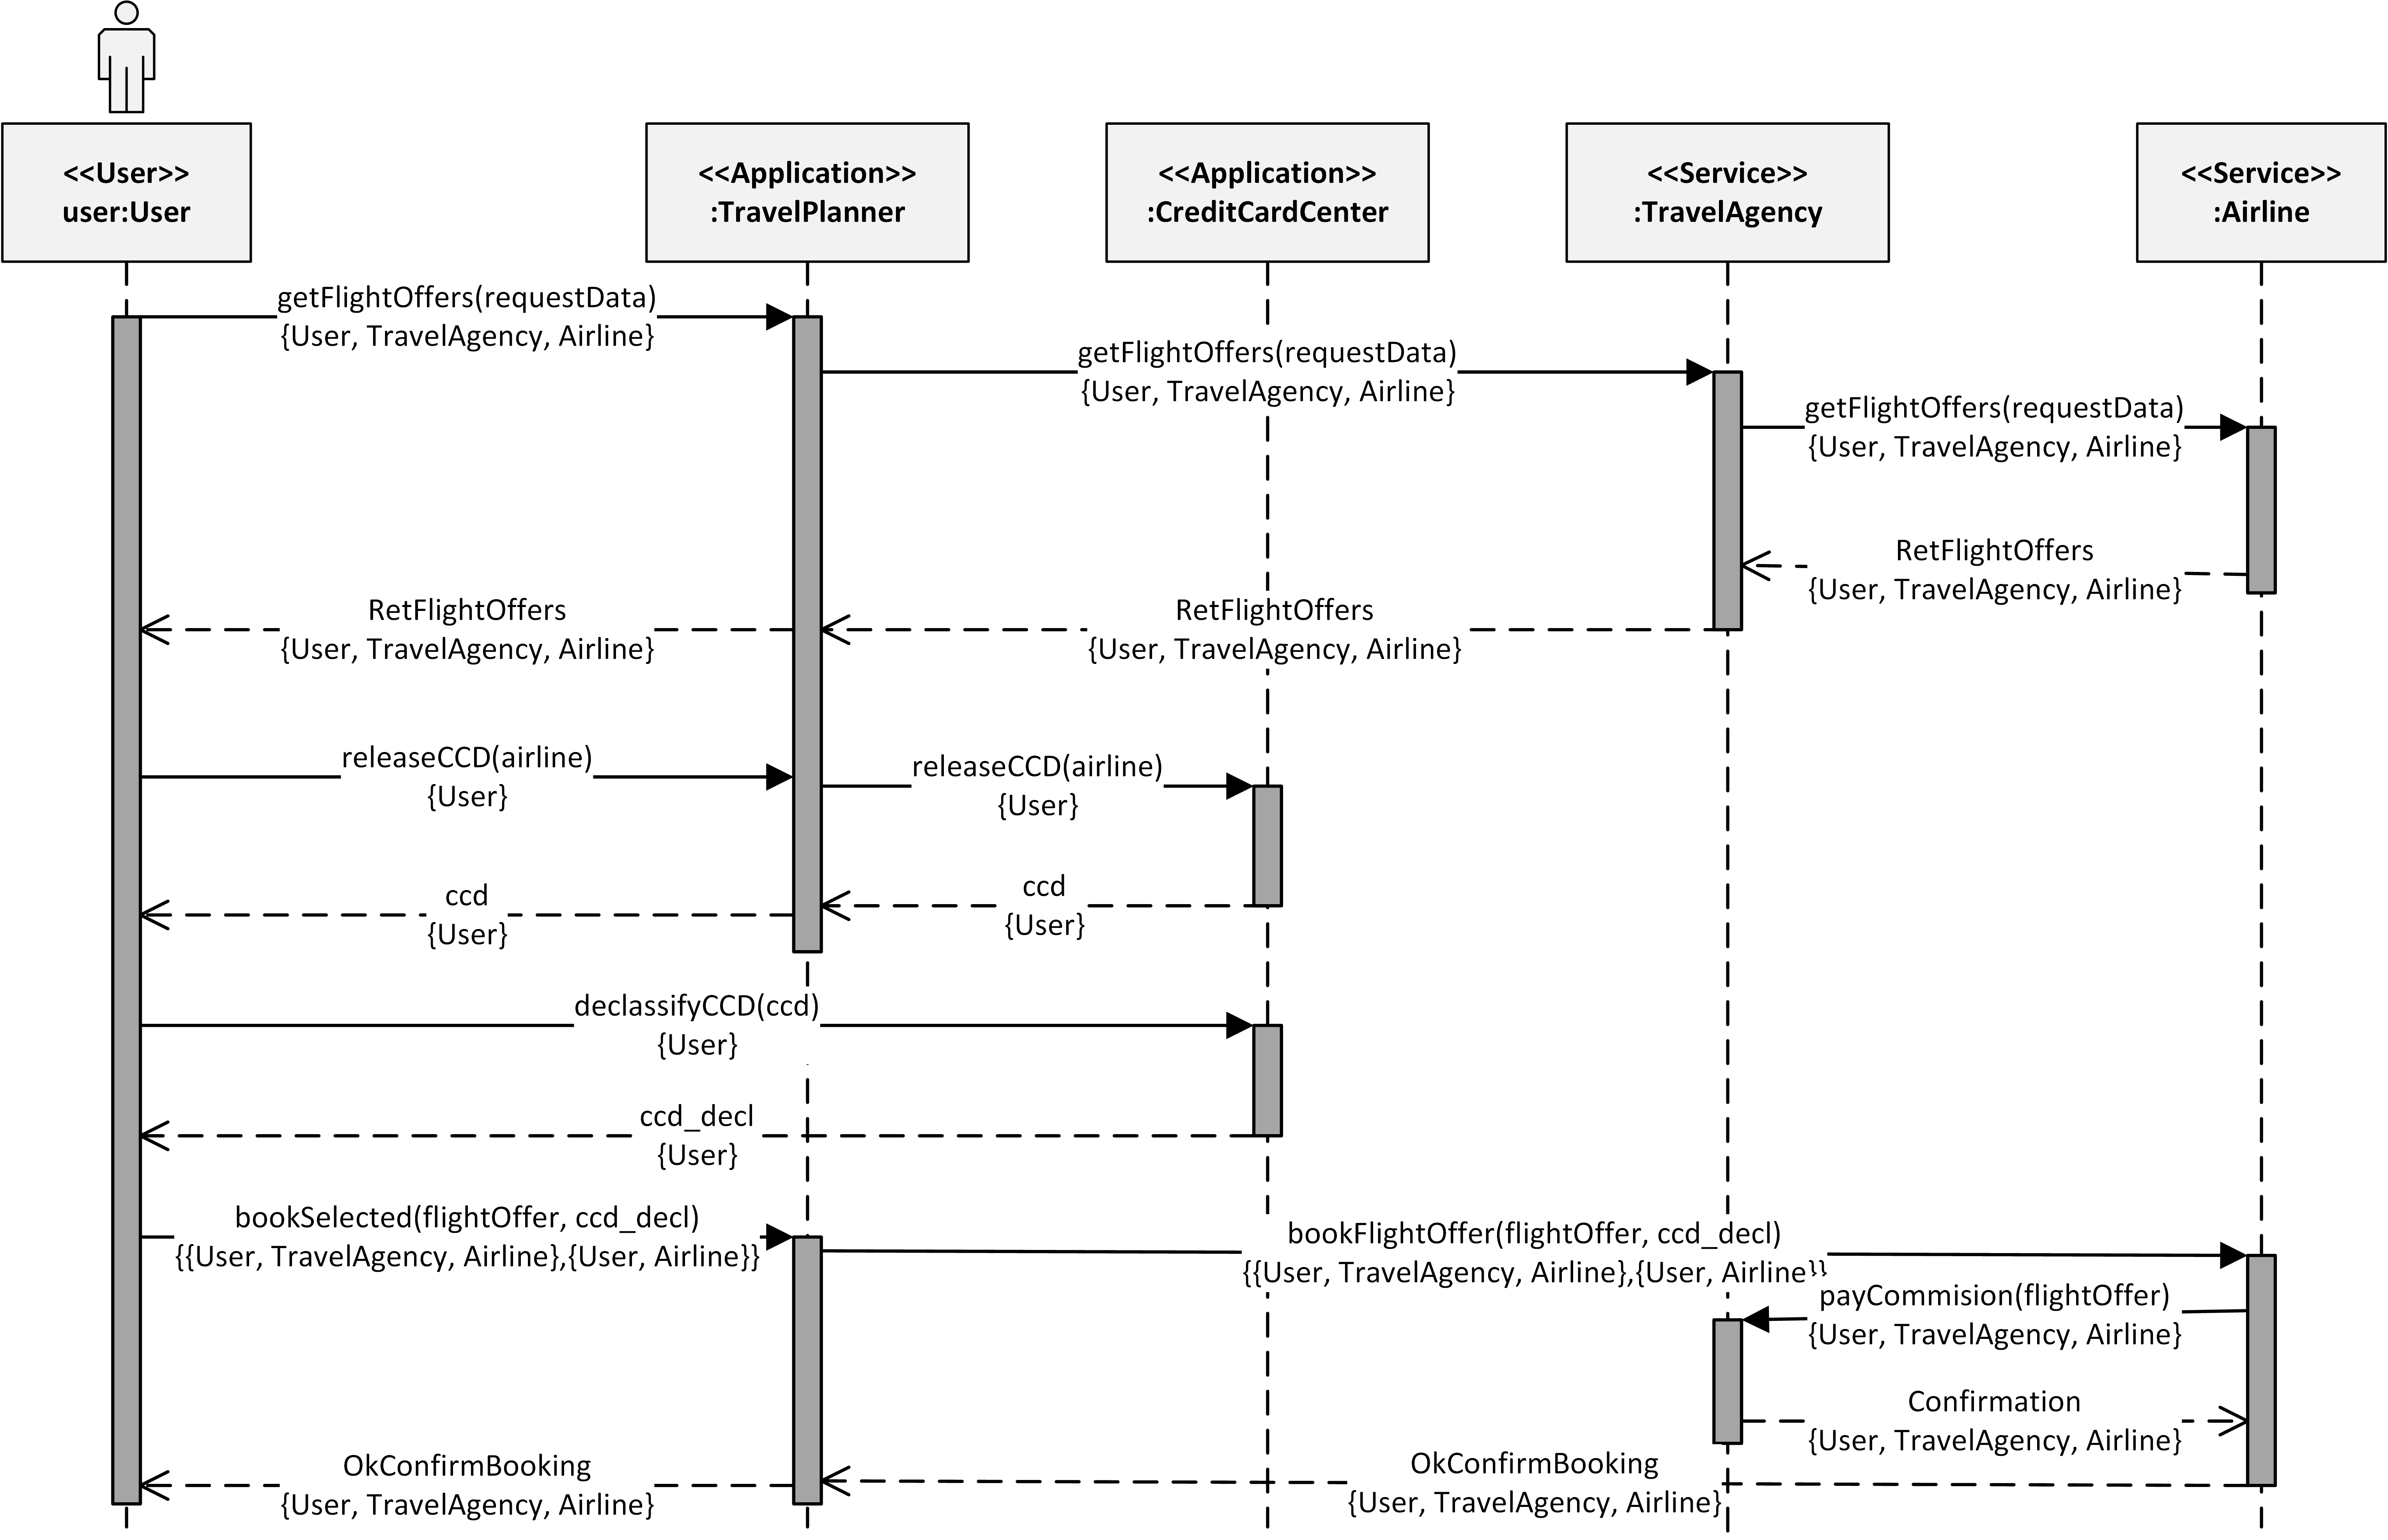
\includegraphics[width=1\textwidth]{images/travelplanner_seq_new.png}
	\caption{Buchung eines Fluges}
	\label{img:travelplanner:seq:new}
\end{figure} \par

\subsection{Beschreibung der PCM-Modelle}
\label{sec:travelplanner:pcm}
In \autoref{img:travelplanner:repo} findet sich die graphische Darstellung des Komponenten-Repository-Modells. Aus den Klassen \texttt{Travelplanner}, \texttt{CreditCardCenter}, \texttt{TravelAgency} und \texttt{Airline} wurde jeweils eine \texttt{BasicComponent}. Die Komponenten kommunizieren über Schnittstellen miteinander. Dabei ist der \texttt{Travelplanner} die zentrale Komponente. Sie kommuniziert über die Schnittstelle \texttt{FlightOffers} mit der \texttt{TravelAgency} und der \texttt{Airline}, um Flüge zu erhalten. Mithilfe der Schnittstelle \texttt{Booking} kann der \texttt{Travelplanner} mit der \texttt{Airline} kommunizieren, um einen Flug zu buchen. Über die Schnittstelle \texttt{Declassification} kann mit der \texttt{CreditCardCenter}-Komponente kommuniziert werden. Mithilfe dieser Schnittstelle kann eine Freigabe der Kreditkartendaten erhalten werden. \par 
Da das Modell nicht vollständig war und nicht zur PCM-Methodik gepasst hat, musste es angepasst und vervollständigt werden. Dazu wurden alle Schnittstellen entfernt, die eine Aktion vom Benutzer als Aufgerufenem statt Aufrufendem gefordert haben. Dazu gehörten die Schnittstellen \texttt{Input} und \texttt{Confirmation}. Damit der Benutzer trotzdem mit dem System interagieren kann wurde die Schnittstelle \texttt{BookingSelection} erweitert. Sie wird vom \texttt{Travelplanner} bereitgestellt. Diese Schnittstelle enthält vier Signaturen, über die der Benutzer mit dem System interagieren kann. Mit \texttt{BookingSelection.bookSelected} kann der Benutzer einen gewünschten Flug, mit seiner Kreditkarte buchen. Mithilfe des Dienstes \texttt{BookingSelection.getFlightOffers} kann der Benutzer Flüge anfordern. Schließlich kann der Benutzer mit \texttt{BookingSelection.releaseCCD} und \texttt{BookingSelection.declass-\\ifyCCD} seine Kreditkartendaten für eine bestimmte Fluglinie anfordern und freigeben. Außerdem wurde in dem Modell die Signatur der Schnittstelle \texttt{Commision} angepasst. Die Signatur \texttt{void payCommision()} wurde in \texttt{bool payCommision(int offerId)} geändert, damit die Fluglinie und Reiseagentur wissen, für was eine Provision gezahlt werden soll. Der geänderte Rückgabetyp signalisiert, ob der Vorgang erfolgreich war. Die Änderungen wurden in \autoref{sec:appendix:travelplanner:old:repo} markiert. \par
\begin{figure}[h]
	\centering
  	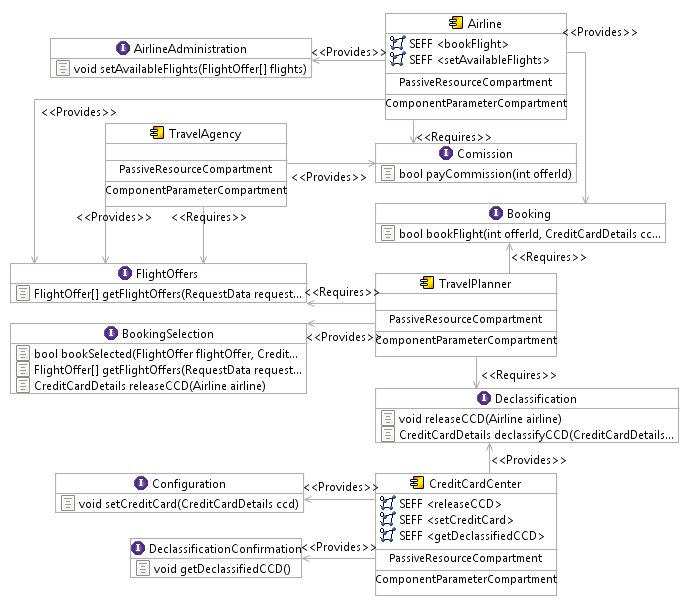
\includegraphics[width=1\textwidth]{images/travelplanner_repository.png}
	\caption{Komponenten-Repository-Modell des Travelplanner}
	\label{img:travelplanner:repo}
\end{figure} 
Die graphische Darstellung des Ressourcen-Umgebungs-Modells ist in \autoref{img:travelplanner:res} abgebildet.
Das Ressourcen-Umgebungs-Modell besteht aus drei \texttt{ResourceContainern} und drei \texttt{LinkingResource}s. Der erste \texttt{ResourceContainer} modelliert ein Handy (\texttt{MobilePhone}). Dieser ist mit dem zweiten \texttt{ResourceContainer}, der einen Server der Fluglinie (\texttt{Airline-\\Server}) modelliert, über zwei der \texttt{LinkingResource}s verbunden. Die Erste modelliert eine 4G- und Internetverbindung (\texttt{4g+Internet}). Die zweite \texttt{LinkingResource} modelliert eine Wlan- und Internetverbindung (\texttt{OpenWifi+Internet}). \texttt{AirlineServer} ist außerdem mit dem dritten \texttt{ResourceContainer} verbunden. Dieser modelliert den Server der Reiseagentur (\texttt{AgencyServer}). \texttt{Travelagency} und \texttt{AirlineServer} sind über eine \texttt{LinkingResource} verbunden, die eine Internetverbindung modelliert (\texttt{Internet}). \par
\begin{figure}[h]
	\centering
  	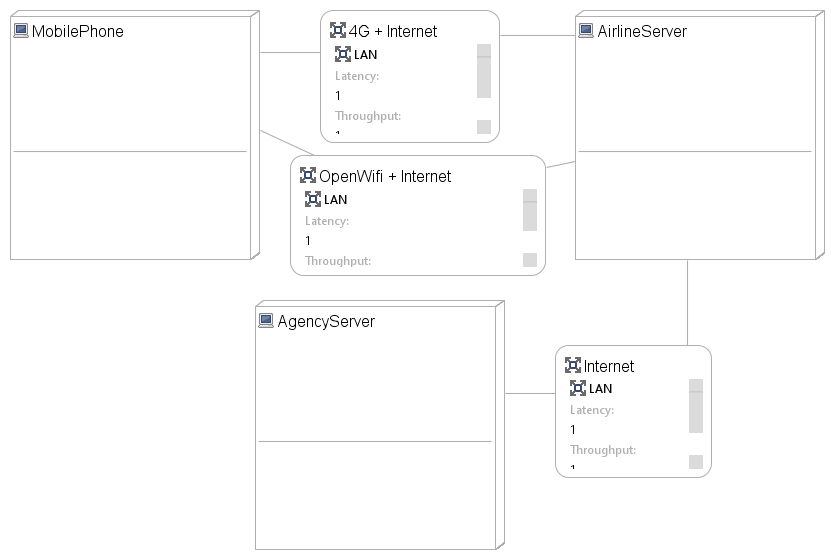
\includegraphics[width=1\textwidth]{images/travelplanner_resource.png}
	\caption{Ressource-Umgebungs-Modell des Travelplanner}
	\label{img:travelplanner:res}
\end{figure} 
Damit das PCM-Modell vervollständigt wird, wurde der TravelPlaner um ein Nutzungsmodell erweitert. Die graphische Darstellung ist in \autoref{img:travelplanner:usage} abgebildet. Das Nutzungsmodell besteht aus vier \texttt{EntryLevelSystemCall}s, die die Benutzerinteraktion aus dem Sequenszdiagramm aus \autoref{img:travelplanner:seq:new} darstellen. Dabei ruft der Benutzer zunächst den Dienst \texttt{BookingSelection.getFlightOffers} auf, um Flüge abzurufen. Im Anschluss gibt der Benutzer seine Kreditkartendaten frei, indem er die beiden Dienste \texttt{Booking-\\Selection.releaseCCD} und \texttt{Declassification.declassify} aufruft. Schließlich bucht er mit dem Aufruf \texttt{Bookingselection.bookSelected} den gewünschten Flug bei der Fluglinie und bezahlt, mit den freigegebenen Kreditkartendaten. \par
\begin{figure}[h]
	\centering
  	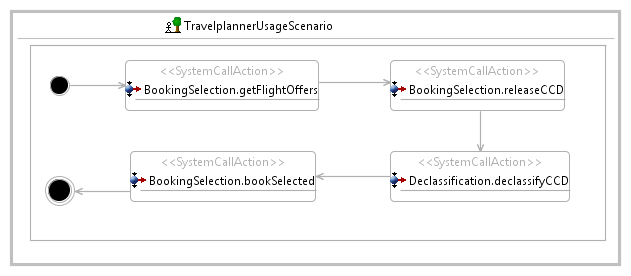
\includegraphics[width=1\textwidth]{images/travelplanner_usage.png}
	\caption{Nutzungsmodell des Travelplanner}
	\label{img:travelplanner:usage}
\end{figure} 
In \autoref{sec:appendix:travelplanner:system} ist das Systemmodell und in \autoref{sec:appendix:travelplanner:allocation} ist das Komponenten-Allokations-Modell des Travelplanner abgebildet. Die Modelle werden in der Transformation und Vertraulichkeitsanalyse verwendet. Sie werden im weiteren Verlauf der Bachelorarbeit nicht diskutiert, da keine Erweiterungen für die Modelle entwickelt wurden.

\subsection{Vertraulichkeitsmodell}
\label{sec:modellierung:confident}
In \cite{Kramera} wurde ein Meta-Modell erstellt, um Vertraulichkeit zu modellieren und später den Datenfluss analysieren zu können. Im Folgenden wird ein Teil dieses Meta-Modells beschrieben. Dieser Teil des Meta-Modells wird benötigt um das Travelplanner-Fallbeispiel zu erweitern, damit es im Anschluss von der Vertraulichkeitsanalyse aus \cite{Kramera} analysiert werden kann.\par
Eines dieser Elemente aus dem Meta-Modell ist \texttt{DataSet}. Ein \texttt{DataSet} modelliert verschiedene Arten von Informationen, die in einem System verarbeitet werden. Die Idee ist, dass man diese \texttt{DataSet}s Akteuren zuordnet. Ein Akteur kann dabei eine Person oder ein System sein. Ein Akteur hat nur Zugriff auf Informationen aus den \texttt{DataSet}s, die ihm zugeordnet wurden. \texttt{DataSet}s können z.B. der Benutzer, die Fluglinie oder die Reiseagentur sein. Mit dem Element \texttt{Location} können Orte für Resource-Container und Linking-Resources spezifiziert werden. Ein Ort kann z.B. der Raum sein, indem sich der Server der Reiseagentur oder der Fluglinie befindet. Das Element \texttt{TamperProtection} erlaubt es einen Sicherheitsmechanismus für Resource-Container und Linking-Resources zu spezifizieren. Mithilfe von \texttt{LocationAndTamperProtectionPair} kann ein Paar aus einer \texttt{Location} und einer \texttt{TamperProtection} spezifiziert werden. So ein Paar kann z.B. der Raum indem der Server der Reiseagentur steht und ein Passwort sein. Da im Fallbeispiel Sicherheitsmechanismen nicht betrachtet werden, wird das Feld für den Sicherheitsmechanismus im Weiteren nicht betrachtet. Schließlich kann mit dem Element \texttt{ParametersAndDataPair} ein Parameter aus dem Komponenten-Repository-Modell mit einem \texttt{DataSet} verknüpft werden. Ein Beispiel für ein solches \texttt{ParametersAndDataPair} könnte der Parameter \textit{ccd}, der die Kreditkartendaten enthält und das \texttt{DataSet} \textit{Benutzer} sein. Das heißt, dass Akteure mit Zugang zu dem \texttt{DataSet} \textit{Benutzer} auch Zugang zu dem Parameter \textit{ccd} haben. \par
%Dieses Element erweitert Resource-Container und Linking-Resources mithilfe von PCM-Profiles. 
Mit diesem Modell, lassen sich Eingabe und Ausgabe eines Systems spezifizieren. Den Datenfluss innerhalb von Komponenten zu modellieren ist, mit dieser Modellierung, nicht möglich. Komponenten werden wie eine Blackbox betrachtet. Bei der Modellierung aus \autoref{ch:modellierung} ist das anders. Dort kann der Datenfluss innerhalb von Komponenten modelliert werden. \par 
Das Vertraulichkeitsmodell enthält außerdem ein Angreifermodell. Ein Angreifer enthält dabei, zu welchem Ort (\texttt{Location}) er Zutritt hat und welche \texttt{DataSet}s ihm zugeordnet wurden. Dadurch kann die Vertraulichkeitsanalyse prüfen, ob jeder Angreifer nur auf die Daten Zugriff hat, auf die er Zugriff haben darf. Ein Angreifer kann z.B. ein Mitarbeiter der Reiseagentur sein, der Zugriff zum Server der Reiseagentur und dem \texttt{DataSet} Reiseagentur hat. Im Rahmen dieser Bachelorarbeit werden Angreifer nicht betrachtet. Deshalb wird das Angreifermodell, aus dem Vertraulichkeitsmodell, für die Validierung, wiederverwendet. \par
Wie bereits bei der Beschreibung der verschiedenen Analysen in \autoref{sec:datenflussanalyse} erwähnt, muss für die Vertraulichkeitsanalyse Eingabe und Ausgabe eines Systems spezifiziert werden. Dazu müssen die Elemente aus dem Vertraulichkeitsmodell in das zu untersuchende System integriert werden. Dies ist mithilfe von MDSDProfiles möglich \cite{Kramer2012}. MDSDProfiles basiert auf EMF-Profiles \cite{EmfProfiles} und erlaubt es das Meta-Modell mit einem Profil zu erweitern, ohne dieses ändern zu müssen.  
Das Profil besteht dabei aus Stereotypen. Ein Stereotyp besteht aus einer Referenz zu einem Element, dass erweitert werden soll und aus einer Referenz zu dem Element, dass erweitern soll. Mithilfe dieser Stereotypen können Elemente durch Annotationen erweitert werden. \par
Die Arbeit von Kramer et. al. \cite{Kramera} bietet ein solches Modell an. Damit ist es möglich das Komponenten-Repository- und das Ressourcen-Umgebungs-Modell mit Elementen aus dem Vertraulichkeitsmodell zu erweitern. Um die Ergebnisse aus der Transformation in die beiden Modelle zu integrieren, benötigt es zwei Stereotypen aus dem Profiles-Modell. Die Beiden sind in \autoref{img:profiles} abgebildet. Mithilfe des \texttt{InformationFlow}-Stereotypen lässt sich das Komponenten-Repository-Modell um einen Informationsfluss erweitern. Dabei können \texttt{ParameterAndDataPair}-Elemente an eine Signatur oder Schnittstelle im Komponenten-Repository-Modell angehängt werden. Der \texttt{LocationAndTamper}-Stereotyp erweitert das Ressourcen-Umgebungs-Modell um eine Zugangsspezifikation. Damit ist es möglich Resource-Container und Linking-Resources im Ressourcen-Umgebungs-Modell mit dem Element \texttt{LocatonAndTamperProtectionPair} zu erweitern . \par
Diese beiden Modelle, das Profiles-Modell und die restlichen PCM-Modelle dienen als Eingabe für die Vertraulichkeitsanalyse. \par
Da eine Modellinstanz der Modellierung aus \autoref{ch:modellierung} durch die Analyse analysiert werden soll, muss diese zunächst transformiert werden. Im Anschluss muss die Transformation mithilfe der Stereotypen aus dem Profiles-Modell mit dem Komponenten-Repository- und Ressourcen-Umgebungs-Modell verknüpft werden. Anschließend kann die Vertraulichkeitsanalyse angewendet werden.
\begin{figure}[h]
	\centering
  	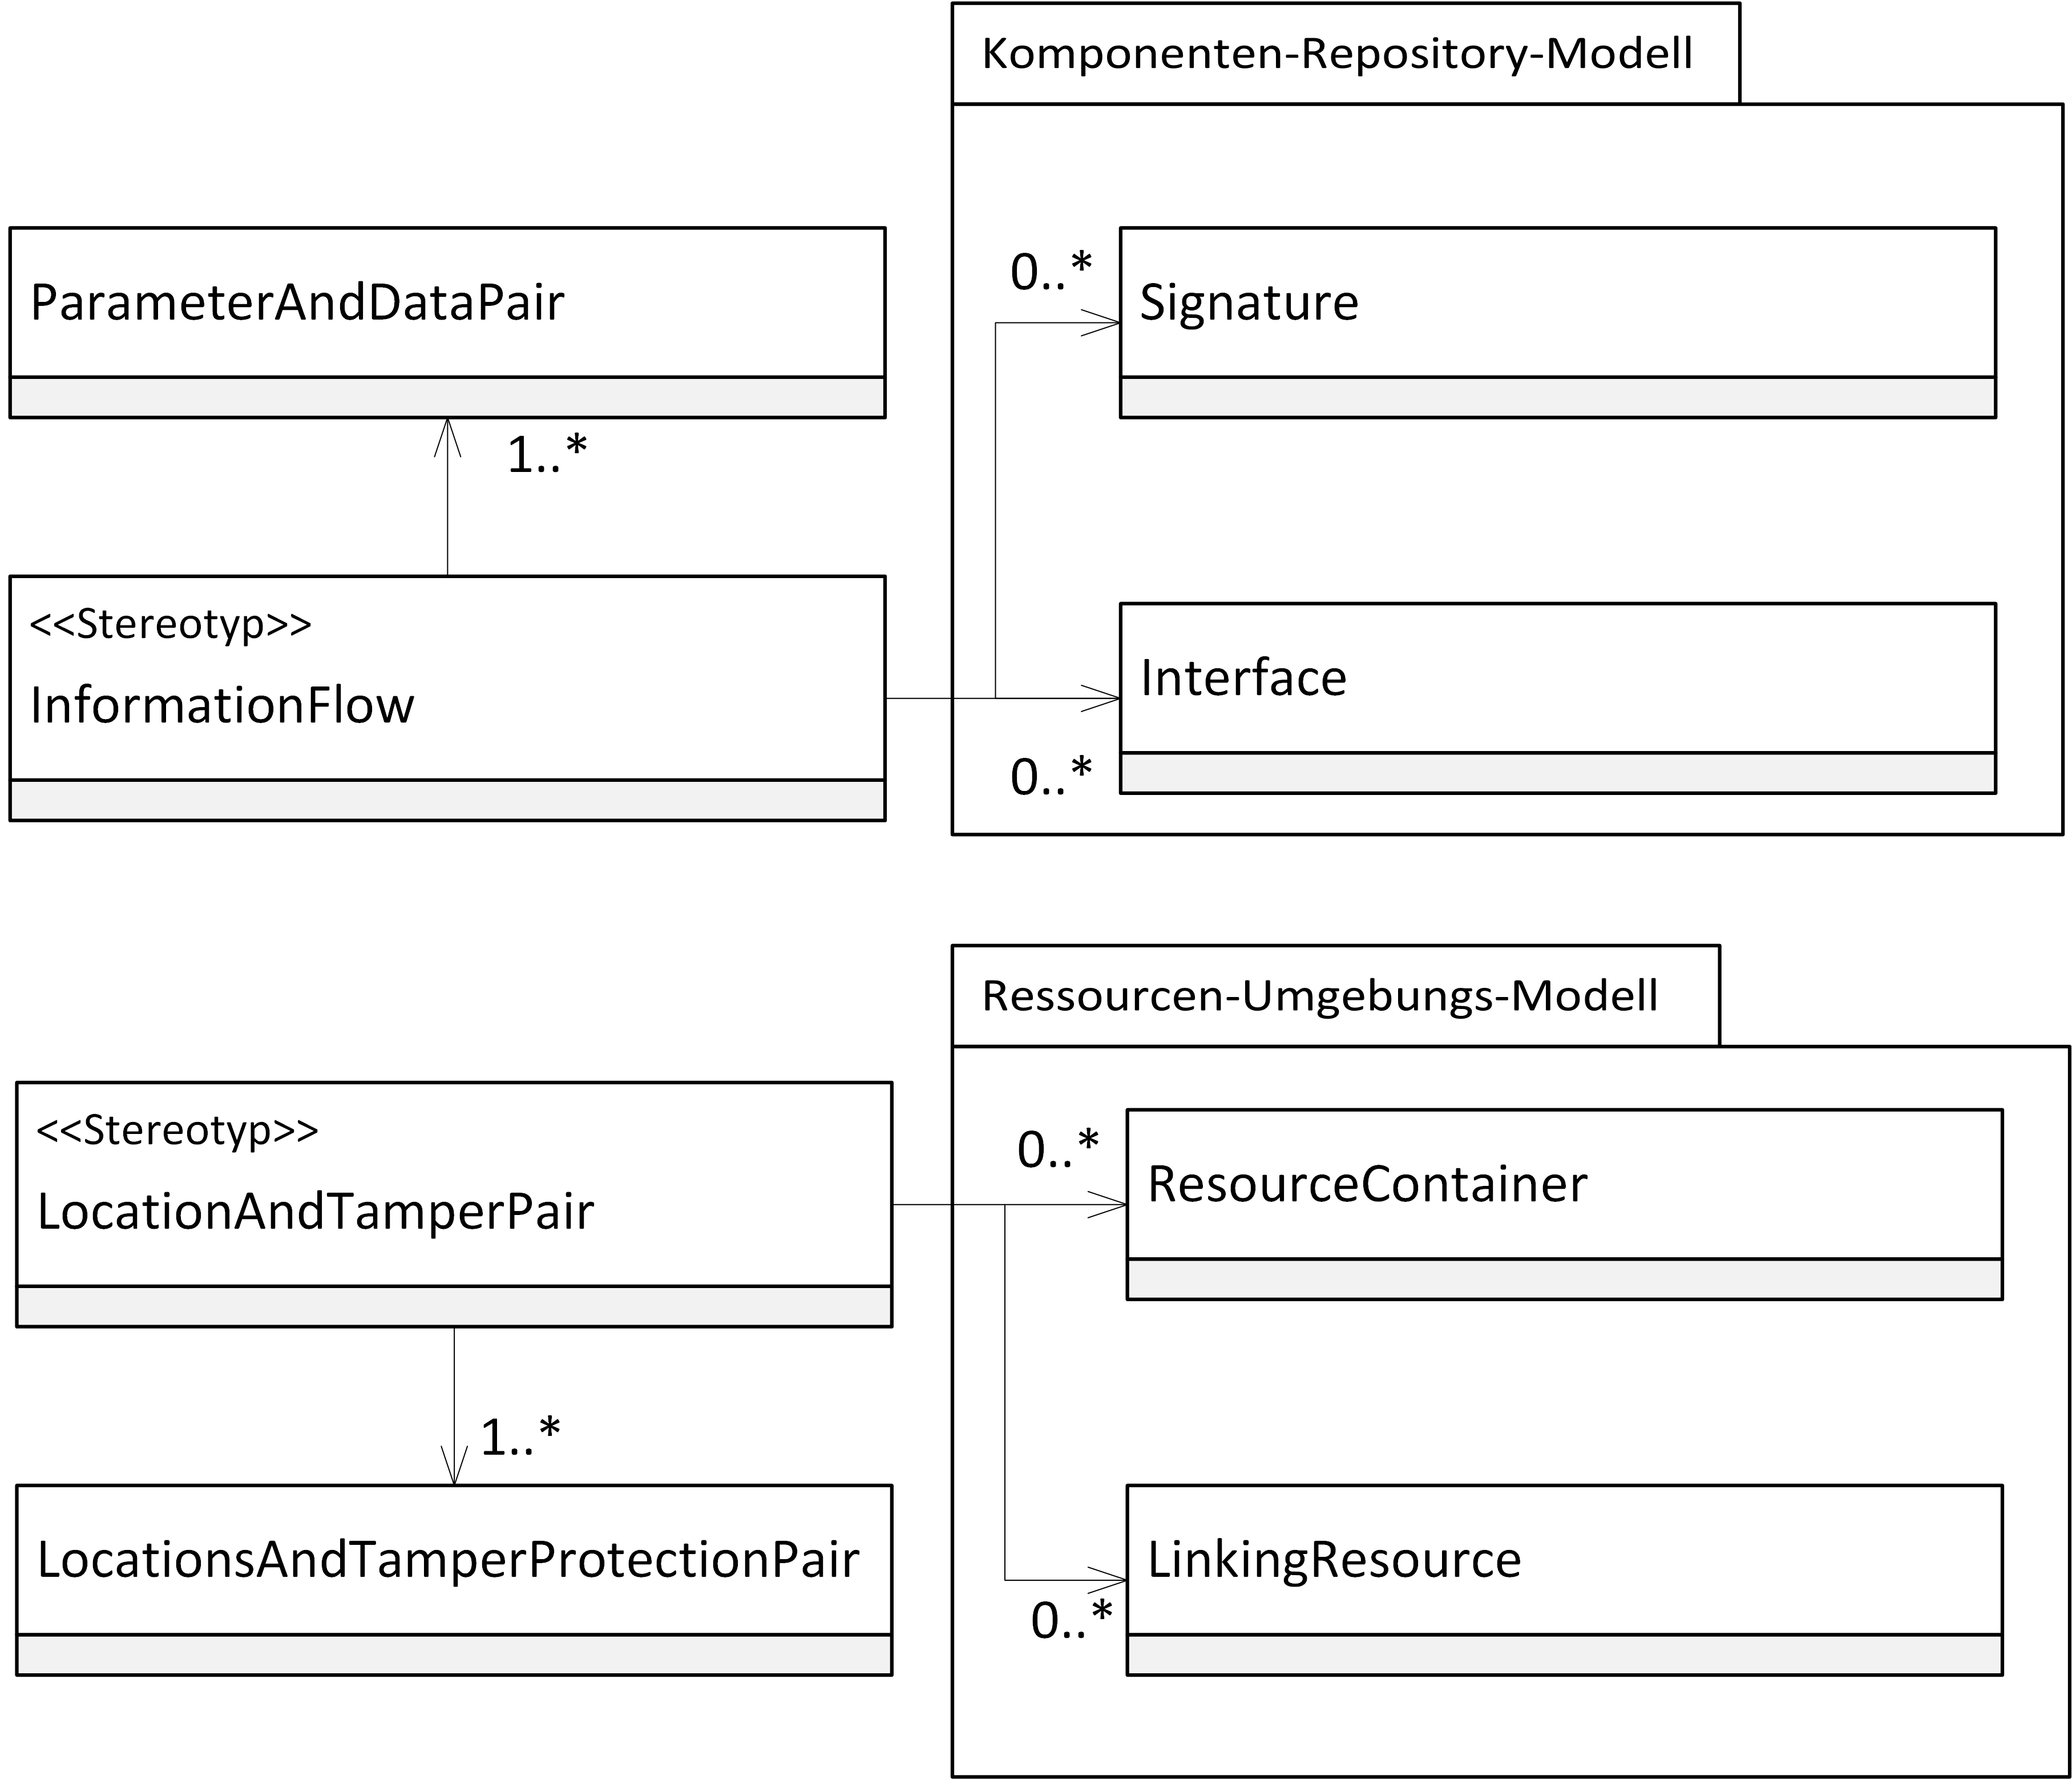
\includegraphics[width=0.6\textwidth]{images/profiles.png}
	\caption{Stereotypen, mit denen das PCM um Elemente, aus dem Vertraulichkeitsmodell, erweitert werden kann}
	\label{img:profiles}
\end{figure}

\subsection{Datenflussmodellierung}
\label{sec:travelplanner:modellierung}
In diesem Abschnitt wird die Daten- und Datenflussmodellierung für den Travelplanner, mit dem in \autoref{ch:modellierung} entwickeltem Meta-Modell, beschrieben. Die Modellierung basiert dabei, auf dem beschriebenen Modell aus \autoref{sec:travelplanner} und der Spezifikation aus \cite{Kramera}. \par
Zunächst wurden für jeden Resource-Container, aus \autoref{img:travelplanner:res}, ein \texttt{ResourceCon-\\tainerPropertyContainer} erstellt, der auf den jeweiligen Resource-Container referenziert. Dabei sind die Resource-Container \texttt{MobilePhone} mit dem Ort \texttt{UserControlled}, der \texttt{AirlineServer} mit dem Ort \texttt{Airline} und \texttt{AgencyServer} mit dem Ort \texttt{Agency} verknüpft. Für die einzelnen Linking-Resources wurden auch jeweils ein \texttt{LinkingResourceProperty-\\Container} erstellt. Dabei sind die Linking-Resources \texttt{4G+Internet} mit dem Ort \texttt{Street} und \texttt{Internet}, \texttt{OpenWifi+Internet} mit dem Ort \texttt{Coffeeshop} und \texttt{Internet} mit dem Ort \texttt{Internet} verknüpft. In \autoref{img:df:rclr} ist die Erweiterung des Resource-Containers \\\texttt{MobilePhone} und der Linking-Resource \texttt{4G+Internet} beispielhaft dargestellt. \par
\begin{figure}[h]
	\centering
  	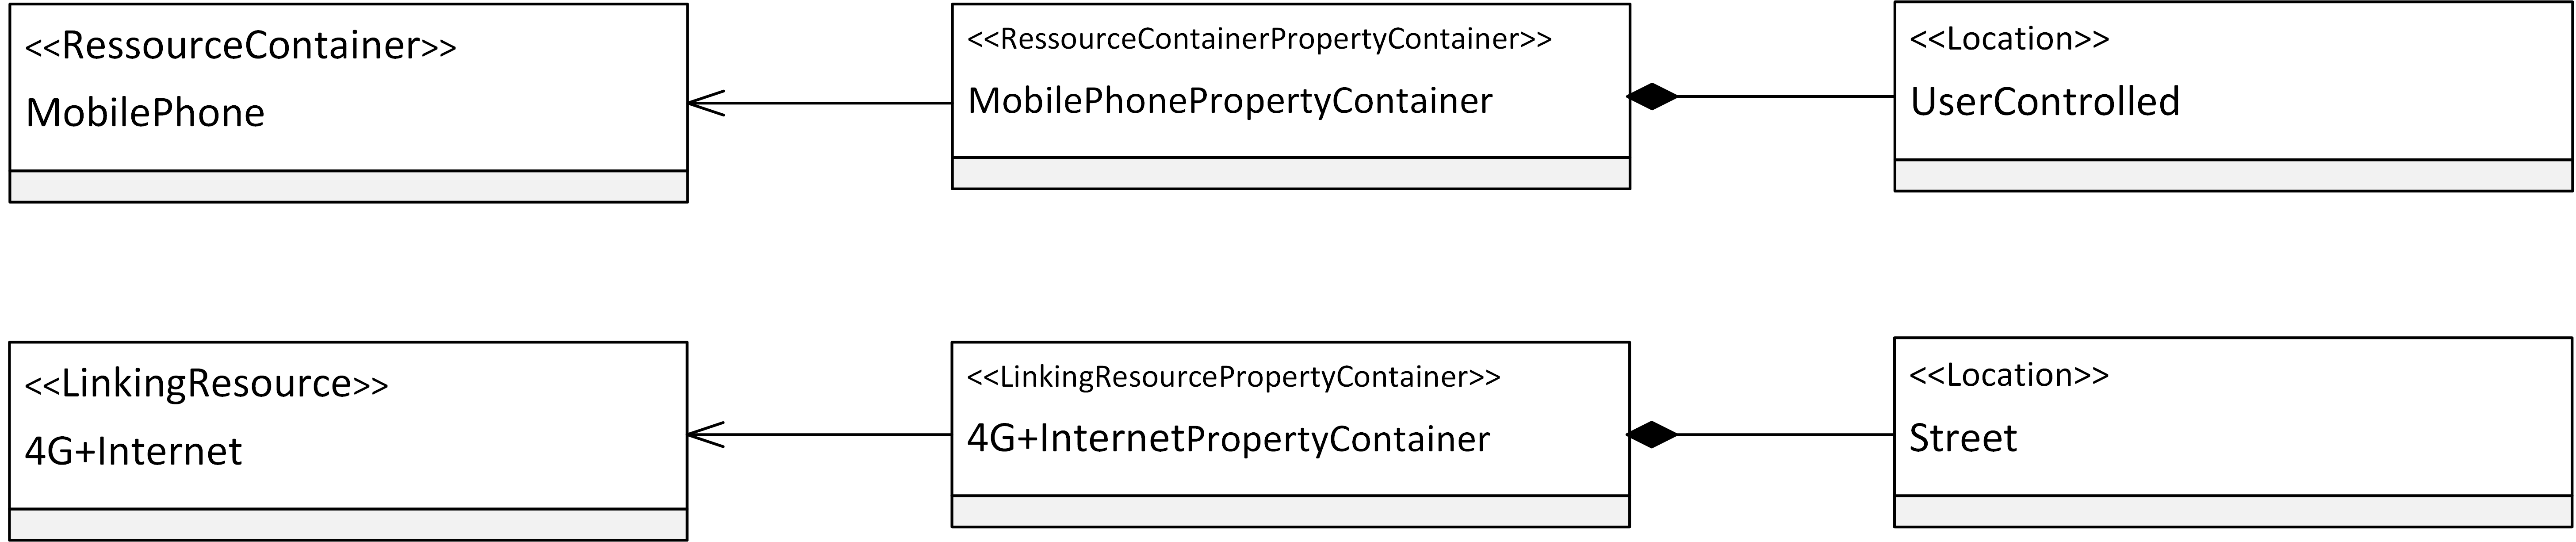
\includegraphics[width=1\textwidth]{images/df_rc_lr.png}
	\caption{Erweiterung von \textit{MobilePhone} und \textit{4G+Internet} um einen Standort}
	\label{img:df:rclr}
\end{figure}
\begin{figure}[h]
	\centering
  	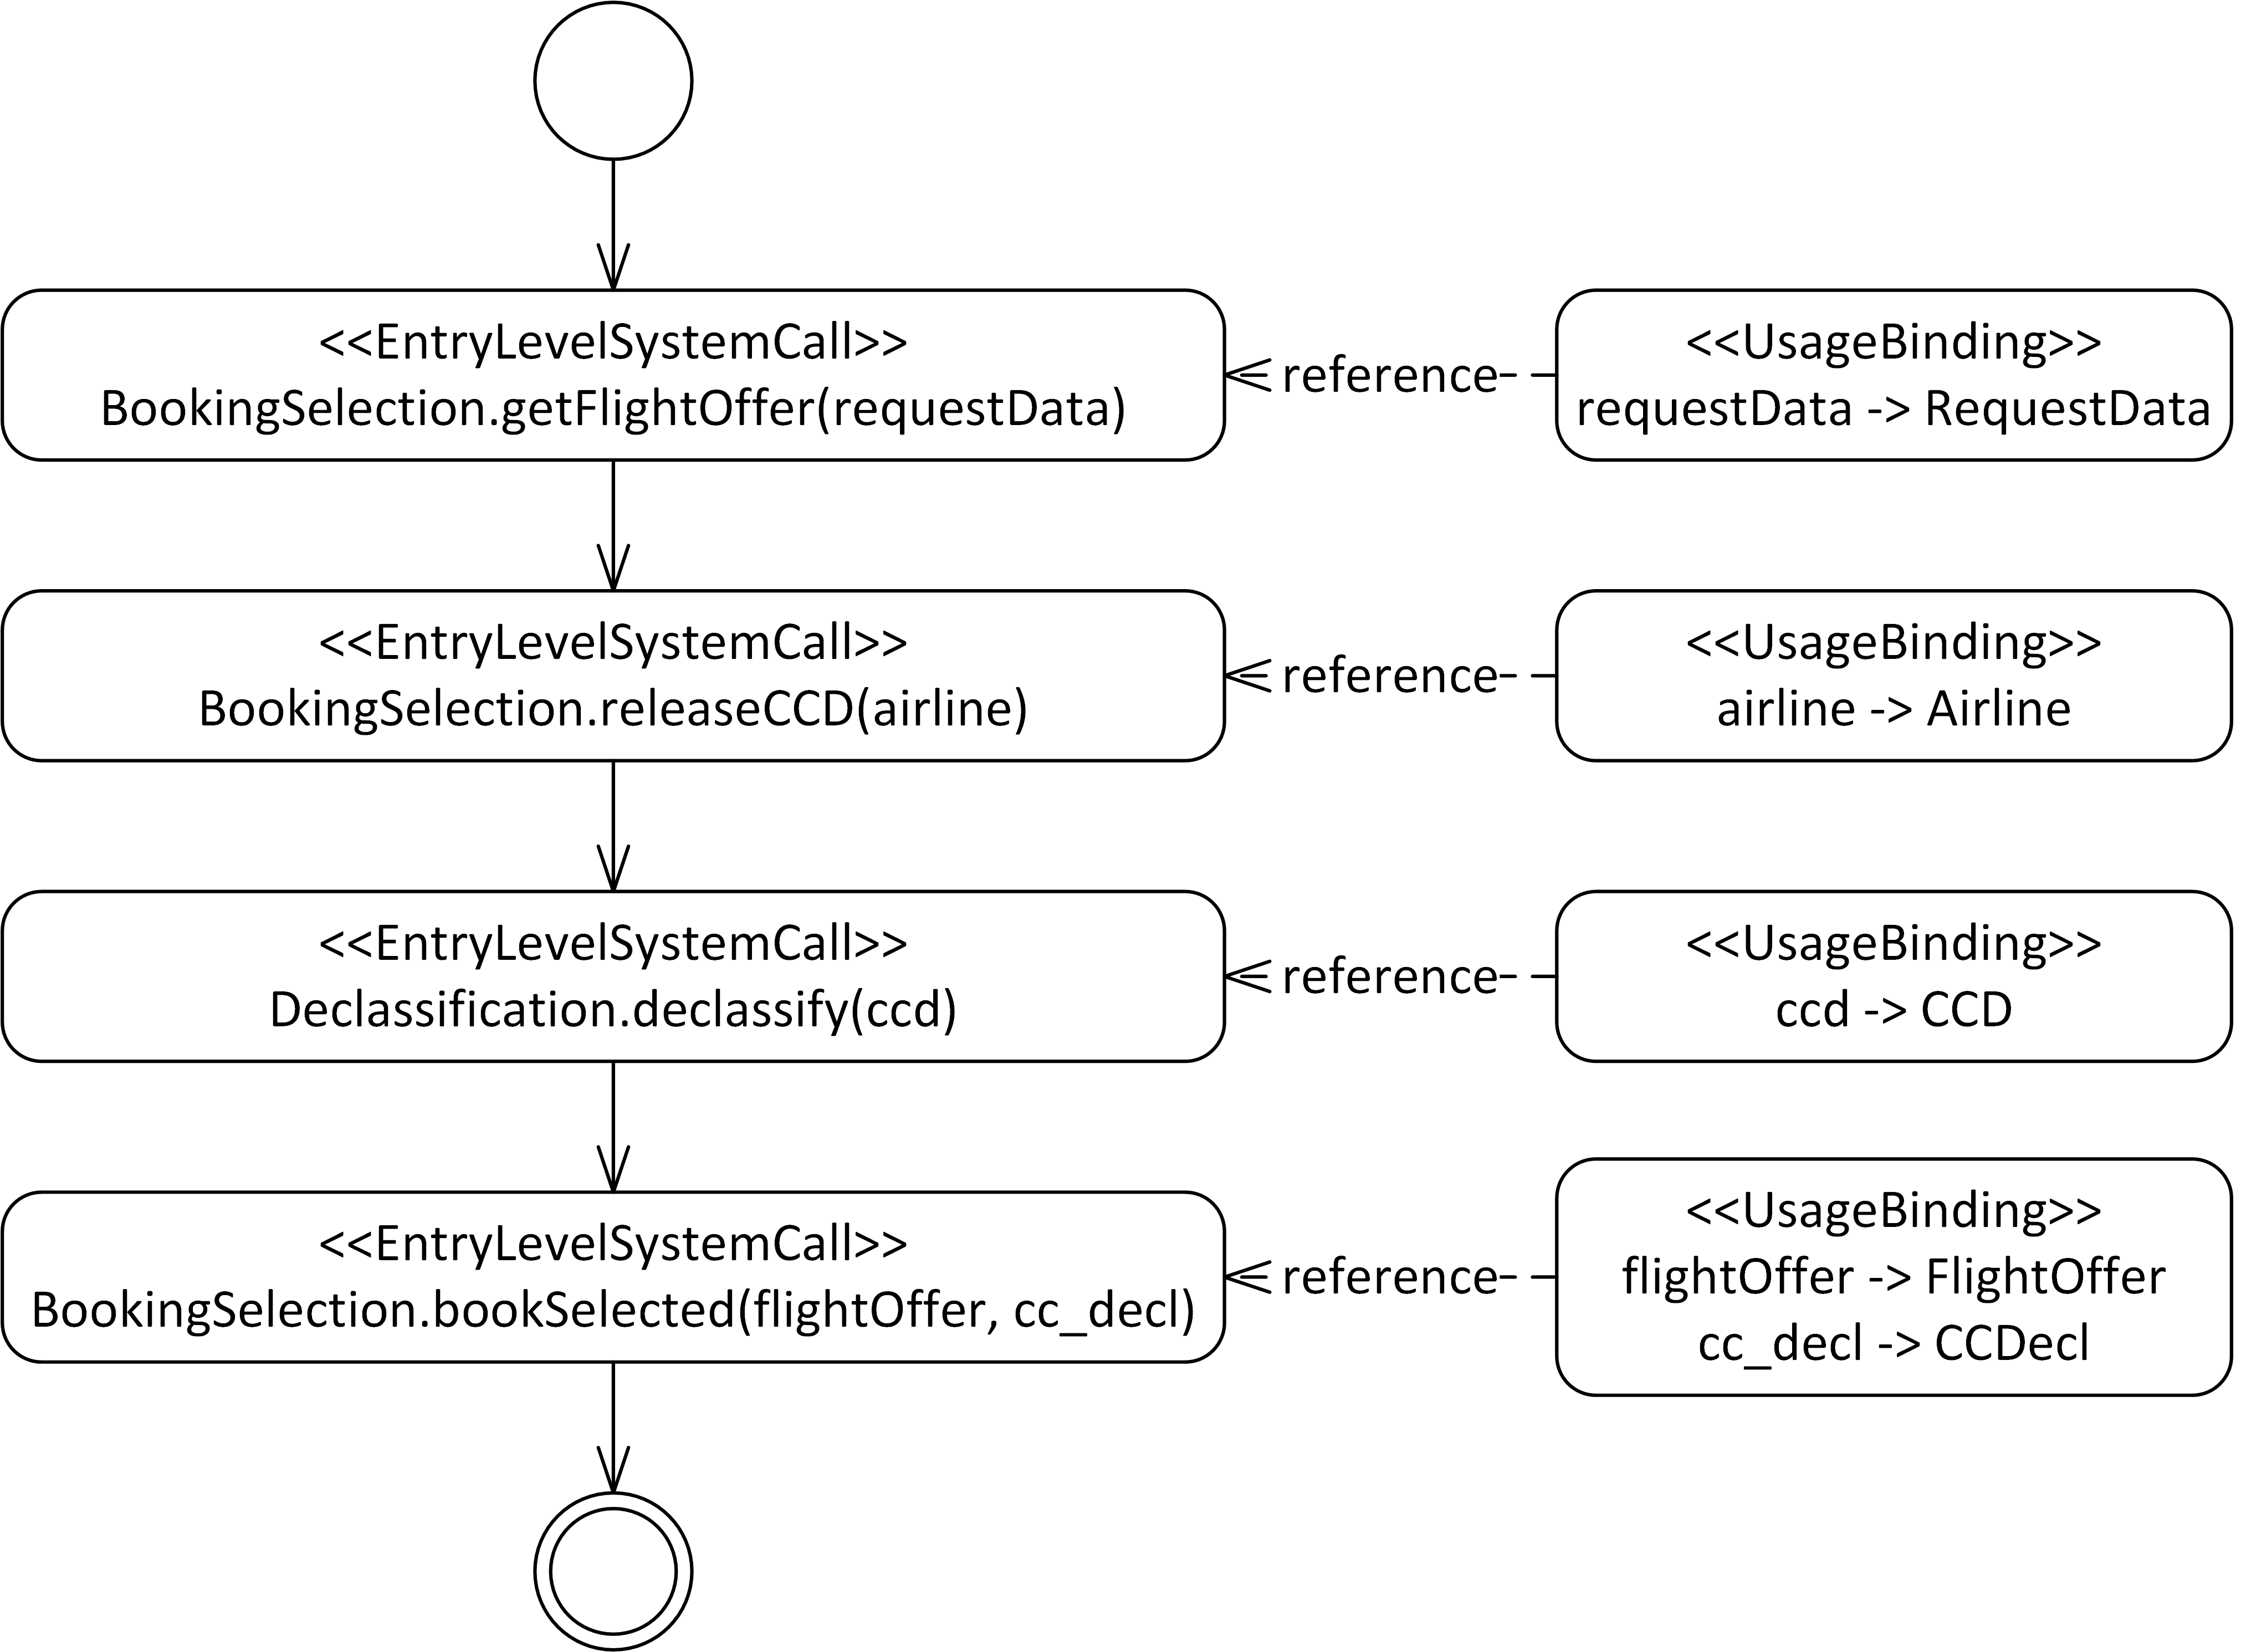
\includegraphics[width=0.8\textwidth]{images/df_usage.png}
	\caption{Erweiterung des Nutzungsmodells um \texttt{Bindings}}
	\label{img:df:usage}
\end{figure}
Als Nächstes wurde mithilfe der Erweiterung für den Domänenexperten, aus Abschnitt \ref{sec:paket:usage}, das Nutzungsmodell um einen Datenfluss erweitert. Dazu wurden die \texttt{EntryLevel-\\SystemCall}s des Nutzungsmodells, aus \autoref{img:travelplanner:usage}, jeweils von einem \texttt{Binding} referenziert. Dabei sind die Parameter aus \texttt{BookingSelection.bookSelected} mit den Datenklassen \texttt{FlightOffer} und \texttt{CCDecl} verknüpft. Der Parameter \textit{requestData} des Dienstes \texttt{BookingSelection.getFlightOffers} ist mit der Datenklasse \texttt{RequestData} verknüpft. Schließlich sind die Parameter der beiden Dienste \texttt{BookingSelection.releaseCCD} und \texttt{Declassification.releaseCCD} mit der Datenklasse \texttt{Airline} verknüpft. In \autoref{img:df:usage} ist die Erweiterung des Nutzungsmodells abgebildet. \par
Mithilfe von \gls{dfseff}s, die in \autoref{sec:paket:dfseff} beschrieben wurden, wurde der Datenfluss innerhalb von Komponenten modelliert und somit das Komponenten-Repository-Modell erweitert. Die Komponente \texttt{Travelplanner} beinhaltet vier \gls{dfseff}s. Der Erste modelliert den Datenfluss innerhalb von \texttt{BookingSelection.getFlightOffers}. Innerhalb des \gls{dfseff}, werden die Daten an den Dienst \texttt{TravelAgency.getFlightOffers} weitergegeben. Dies wird mit einer \texttt{DataFlowExternalAction} modelliert. Sie enthält ein \texttt{Binding}, das den Parameter \textit{requestData} mit der Datenklasse \textit{RequestData} verknüpft. Im Anschluss wird mit \texttt{CreateData} das Rückgabedatum \textit{FlightOfferReturn} erstellt. \autoref{img:df:bookingSelection:getFlight} veranschaulicht das Verhalten. \par
\begin{figure}[h]
	\centering
  	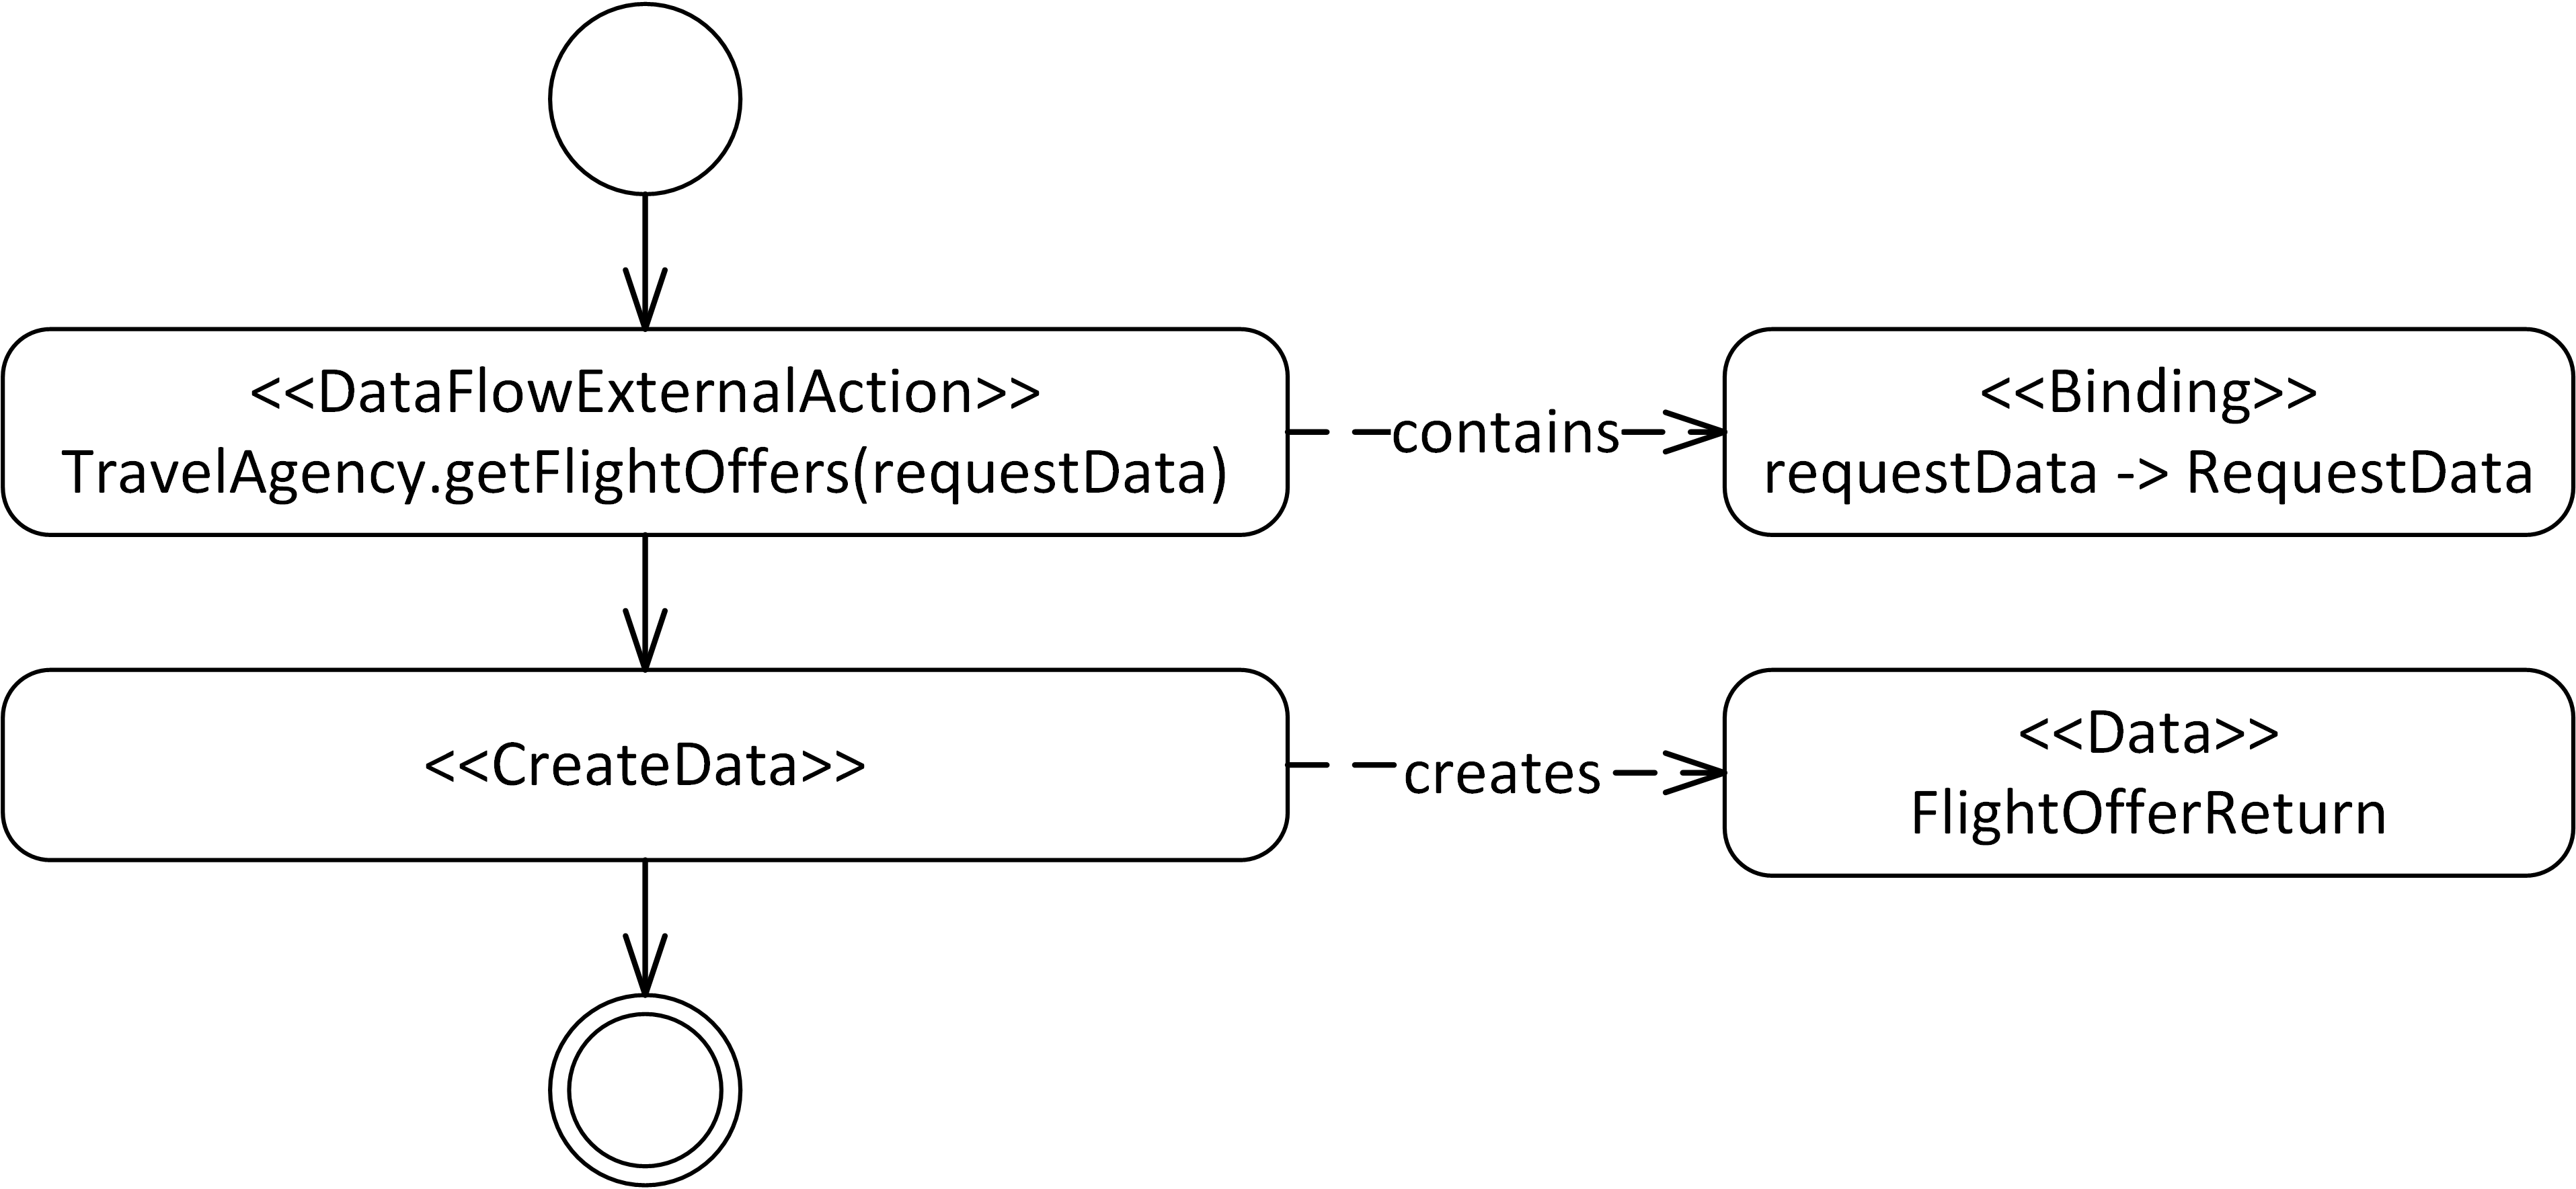
\includegraphics[width=0.7\textwidth]{images/dfseff_bookingSelection_getFlight.png}
	\caption{DFSEFF des Aufrufs \texttt{BookingSelection.getFlightOffers}}
	\label{img:df:bookingSelection:getFlight}
\end{figure}
Der Datenfluss innerhalb von \texttt{TravelAgency.getFlightOffers} wird in einem \gls{dfseff} in \texttt{TravelAgency} modelliert. Der Aufruf des Dienstes \texttt{Airline.getFlightOffers} wird, auch hier, mit einer \texttt{DataFlowExternalAction} modelliert. Sie enthält ein \texttt{Binding}, das den Parameter \textit{requestData} mit der Datenklasse \textit{RequestData} verknüpft. Im Anschluss wird mit \texttt{CreateDataAction} das Rückgabedatum \textit{FlightOfferReturn} erstellt. Das Verhalten ist in \autoref{img:df:ta:getFlight} abgebildet. \par
\begin{figure}[h]
	\centering
  	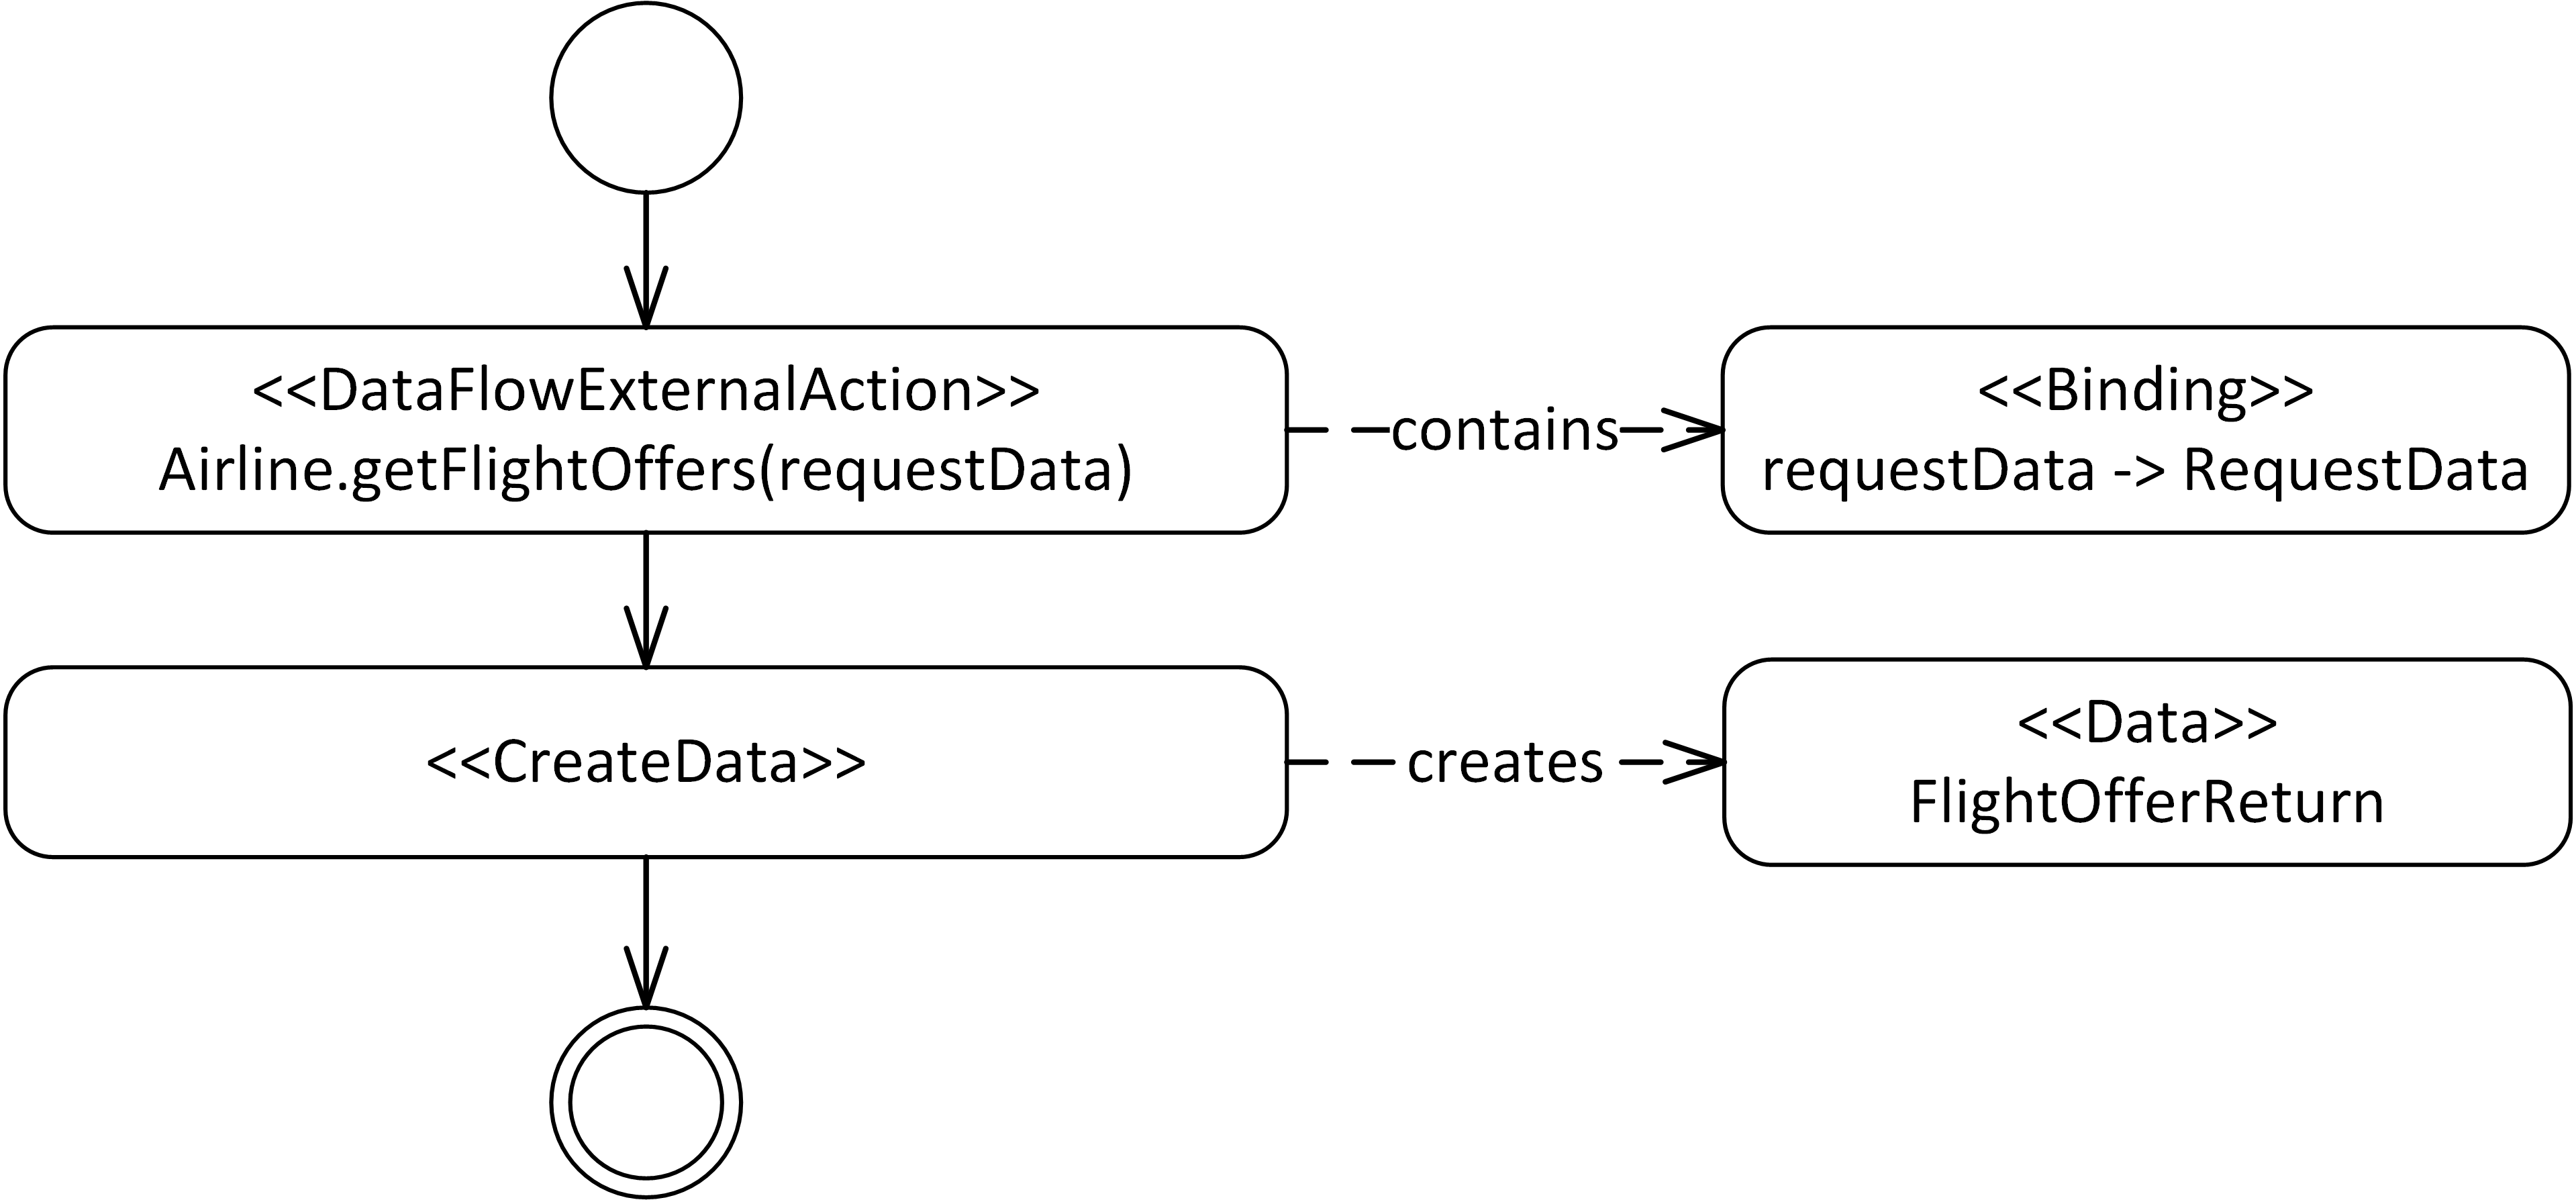
\includegraphics[width=0.7\textwidth]{images/dfseff_TA_getFlight.png}
	\caption{DFSEFF des Aufrufs \texttt{TravelAgency.getFlightOffers}}
	\label{img:df:ta:getFlight}
\end{figure} 
Der zweite \gls{dfseff}, im Travelplanner, modelliert den Datenfluss innerhalb des Dienstes \texttt{BookingSelection.releaseCCD}. Der Aufruf des Dienstes \texttt{CreditCardCenter.releaseCCD} wird mithilfe einer \texttt{DataFlowExternalAction} modelliert. Sie enthält ein \texttt{Binding}, das den Parameter \textit{airline} mit der Datenklasse \textit{Airline} verknüpft. Daraufhin wird mit \texttt{CreateData} das Rückgabedatum \textit{CCD} erstellt. In \autoref{img:df:bookingSelection:releaseCCD} wird dieses Verhalten veranschaulicht. \par
\begin{figure}[h]
	\centering
  	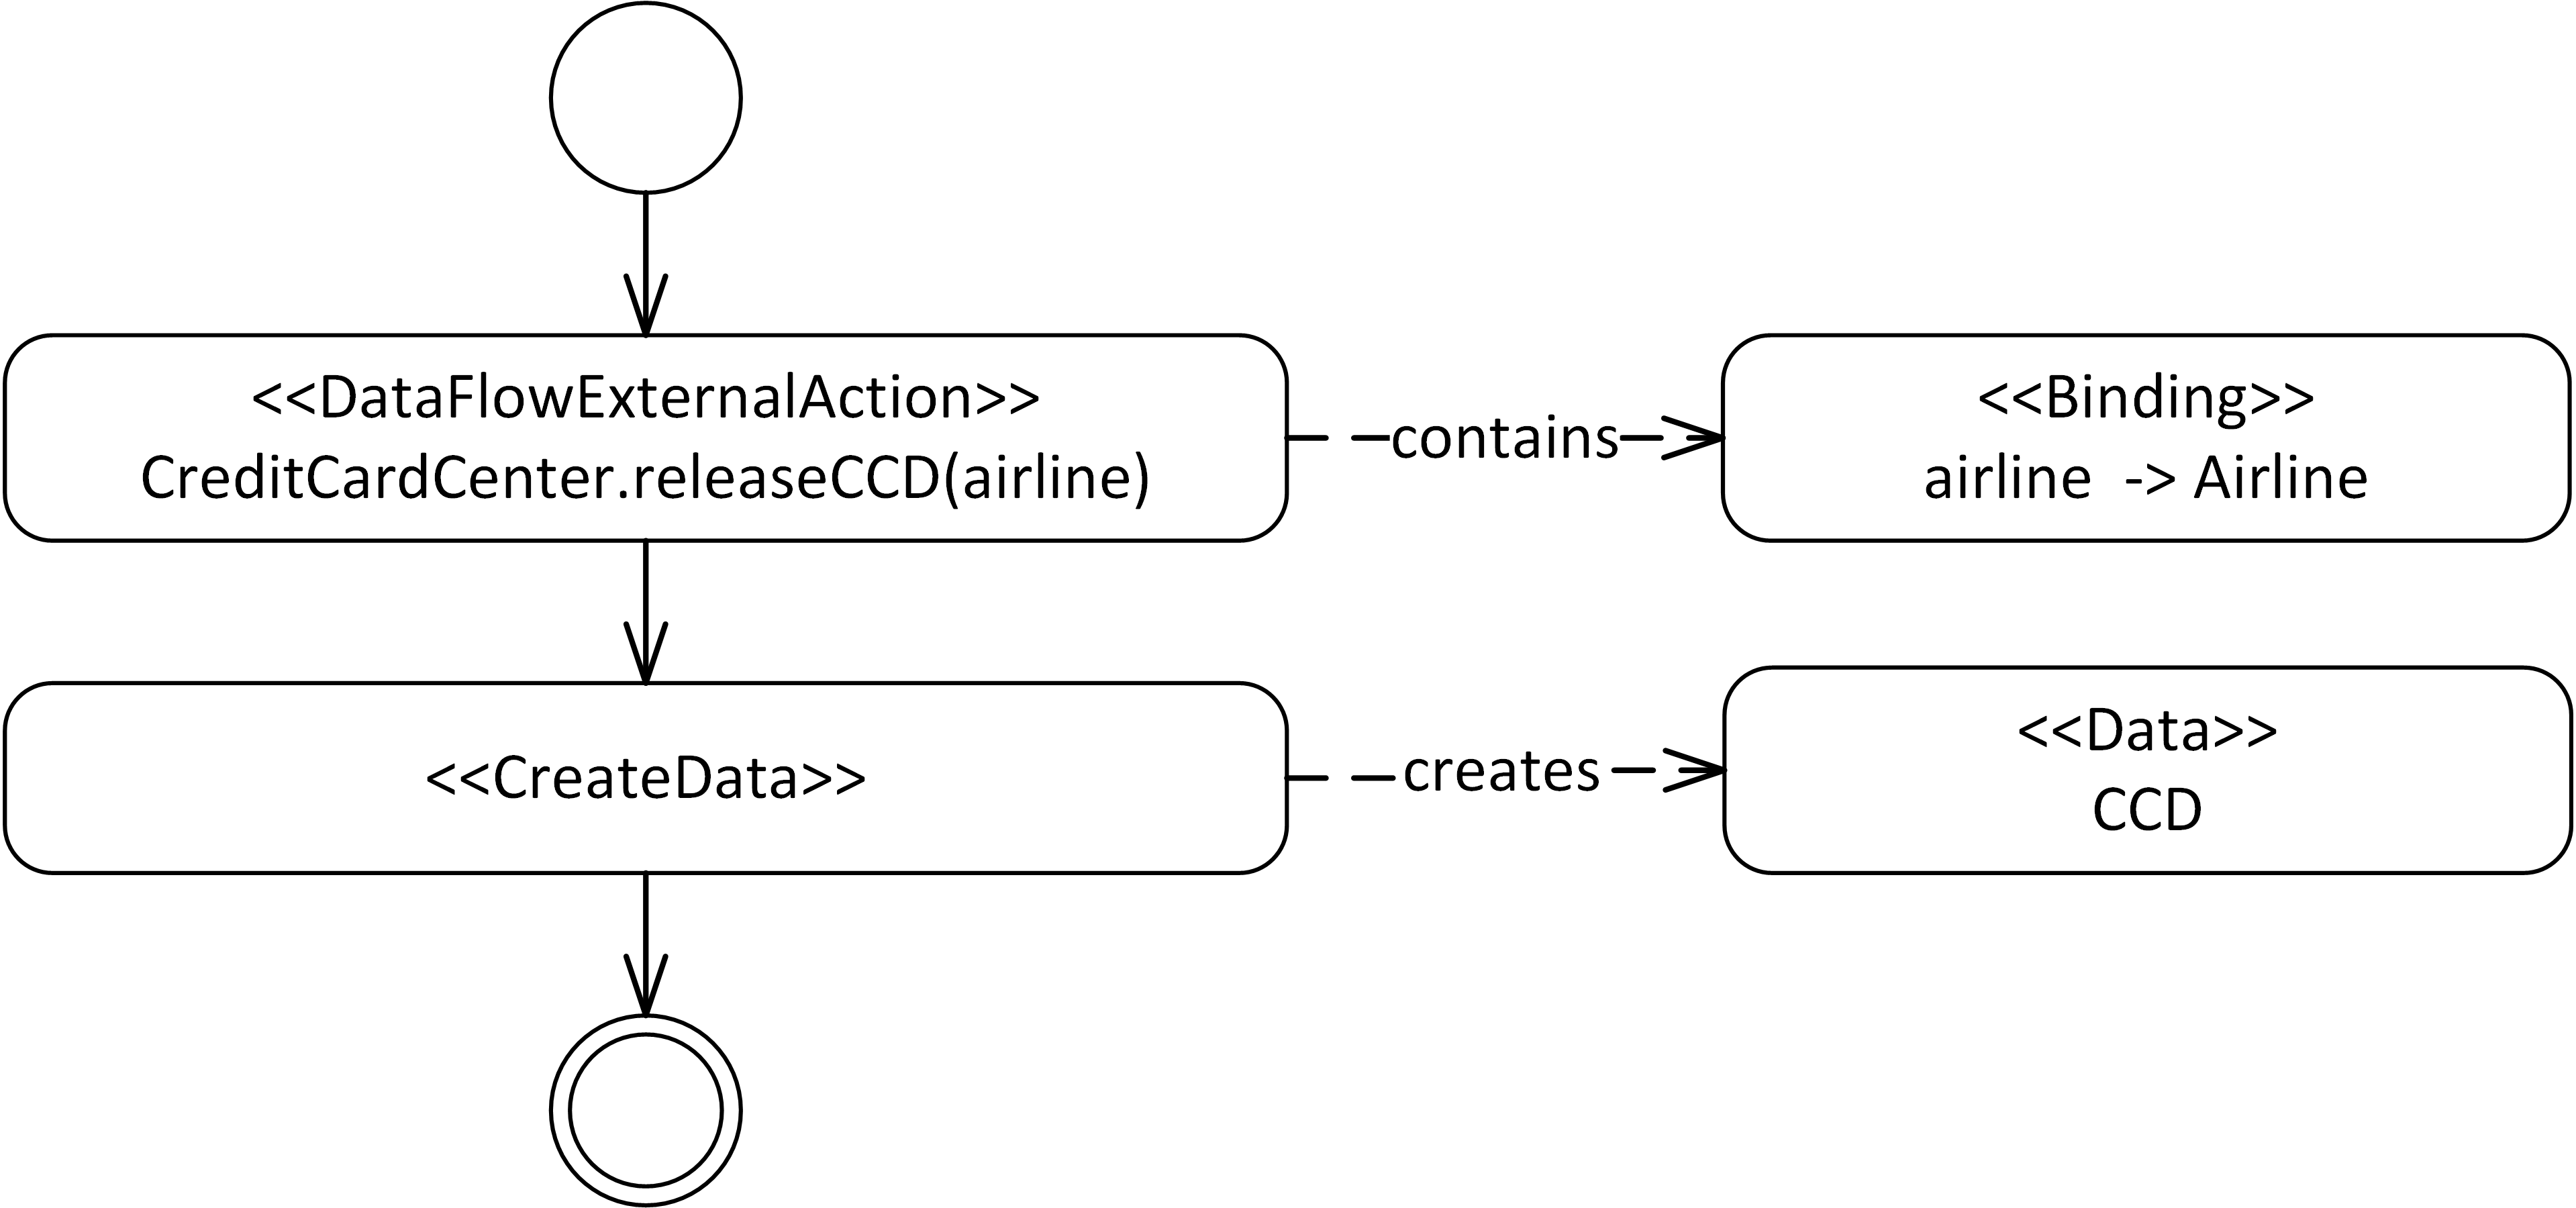
\includegraphics[width=0.7\textwidth]{images/dfseff_bookingSelection_releaseCCD.png}
	\caption{DFSEFF des Aufrufs \texttt{BookingSelection.releaseCCD}}
	\label{img:df:bookingSelection:releaseCCD}
\end{figure}
Im dritten \gls{dfseff} des Travelplanner, wird der Datenfluss innerhalb des Dienstes \\\texttt{Declassification.declassifyCCD} modelliert. Dabei wird mit \texttt{CreateData} das Rückgabedatum \textit{CCDecl} erstellt. Eine Veranschaulichung des Verhaltens ist in \autoref{img:df:ccc:declassify} abgebildet. \par
\begin{figure}[h]
	\centering
  	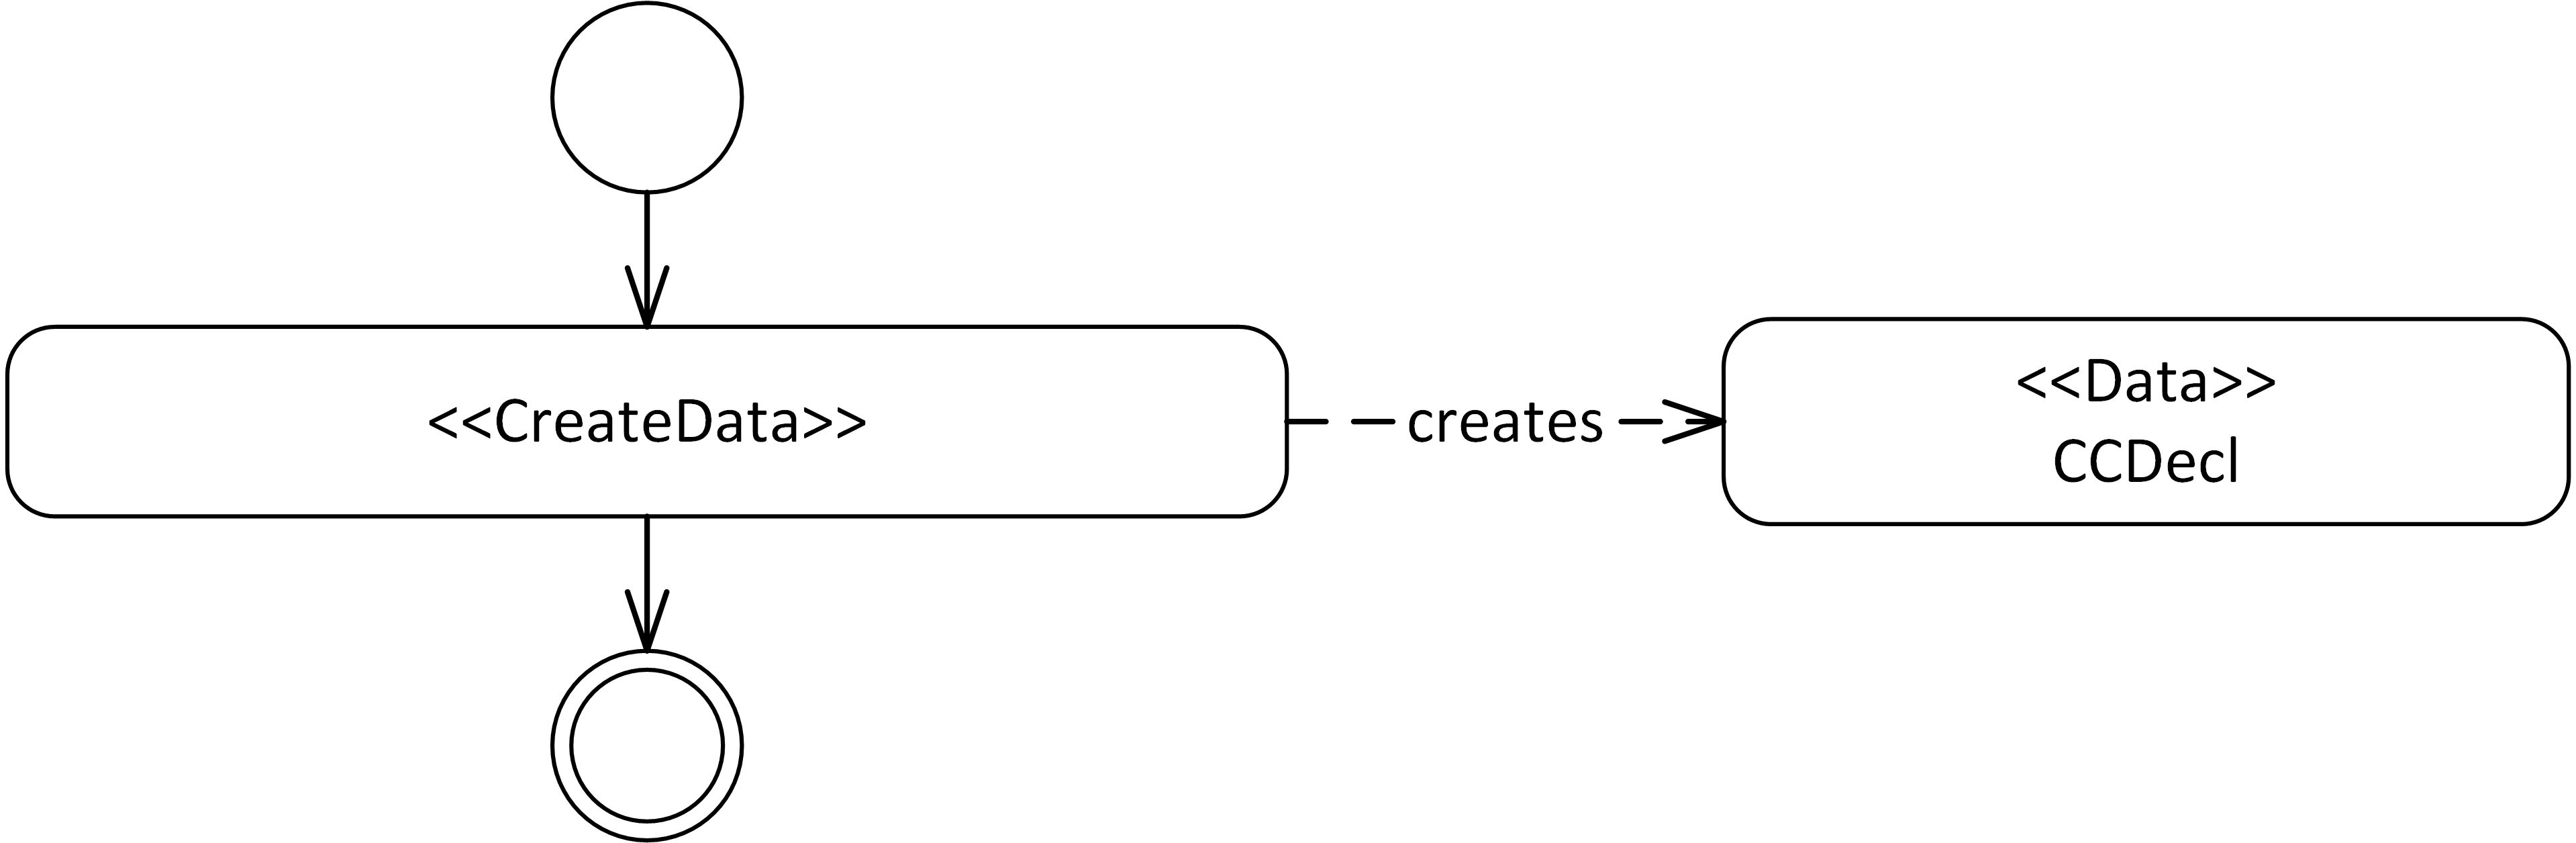
\includegraphics[width=0.7\textwidth]{images/dfseff_CCC_declassify.png}
	\caption{DFSEFF des Aufrufs \texttt{Declassification.declassifyCCD}}
	\label{img:df:ccc:declassify}
\end{figure}
Im vierten und letzten \gls{dfseff} des Travelplanner wird der Datenfluss innerhalb von \texttt{BookingSelection.bookSelected} modelliert. Der Aufruf des Dienstes \texttt{Airline.book-\\FlightOffer} wird mithilfe einer \texttt{DataFlowExternalAction} modelliert. Sie enthält zwei \texttt{Binding}s. Das Erste verknüpft den Parameter \textit{flightOffer} mit der Datenklasse \textit{FlightOffer} und das Zweite verknüpft den Parameter \textit{ccd\_decl} mit der Datenklasse \textit{CCDecl}. Schließlich wird mit \texttt{CreateData} das Rückgabedatum \textit{BookingConfirmation} erstellt. Das Verhalten ist in \autoref{img:df:bookingSelection:bookSelected} abgebildet. \par
\begin{figure}[h]
	\centering
  	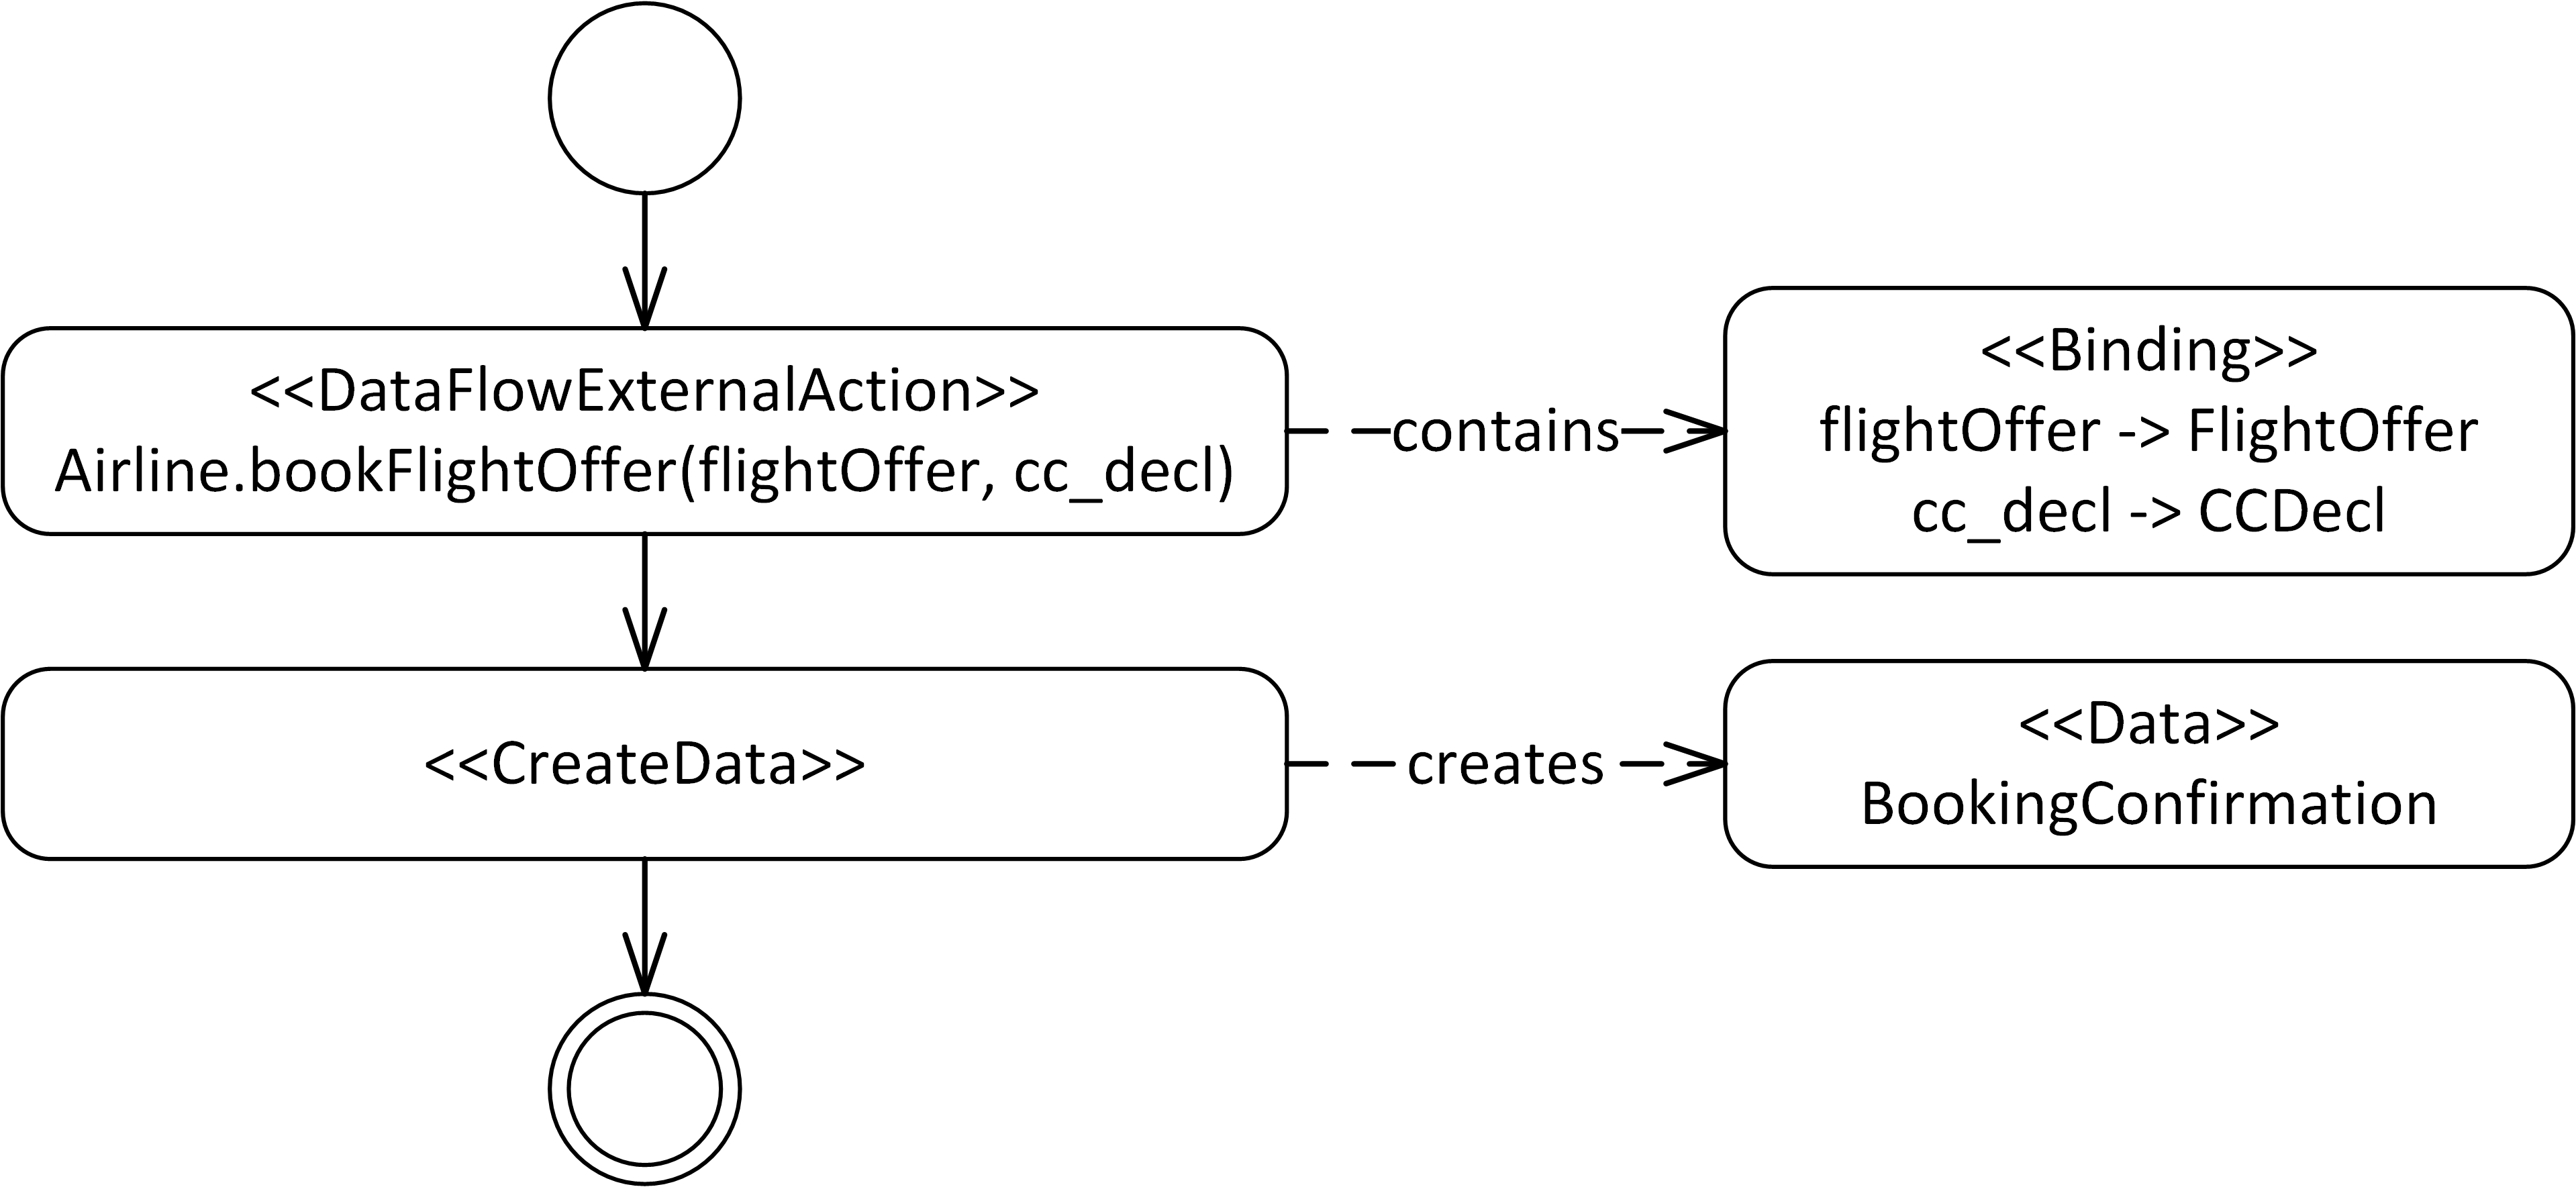
\includegraphics[width=0.7\textwidth]{images/dfseff_bookingSelection_bookSelected.png}
	\caption{DFSEFF des Aufrufs \texttt{BookingSelection.bookSelected}}
	\label{img:df:bookingSelection:bookSelected}
\end{figure}
Der letzte \gls{dfseff} der Modellierung, beschreibt den Datenfluss innerhalb des Dienstes \texttt{Booking.bookFlight}. Der Aufruf des Dienstes \texttt{TravelAgency.payCommision} wird mit einer \texttt{DataFlowExternalAction} modelliert. Sie enthält ein \texttt{Binding}, das den Parameter \textit{flightOffer} mit der Datenklasse \textit{FlightOffer} verknüpft. Mit \texttt{CreateData} wird im Anschluss das Rückgabedatum \textit{BookingConfirmation} erstellt. In \autoref{img:df:booking:bookFlight} ist das Verhalten veranschaulicht.\par
\begin{figure}[h]
	\centering
  	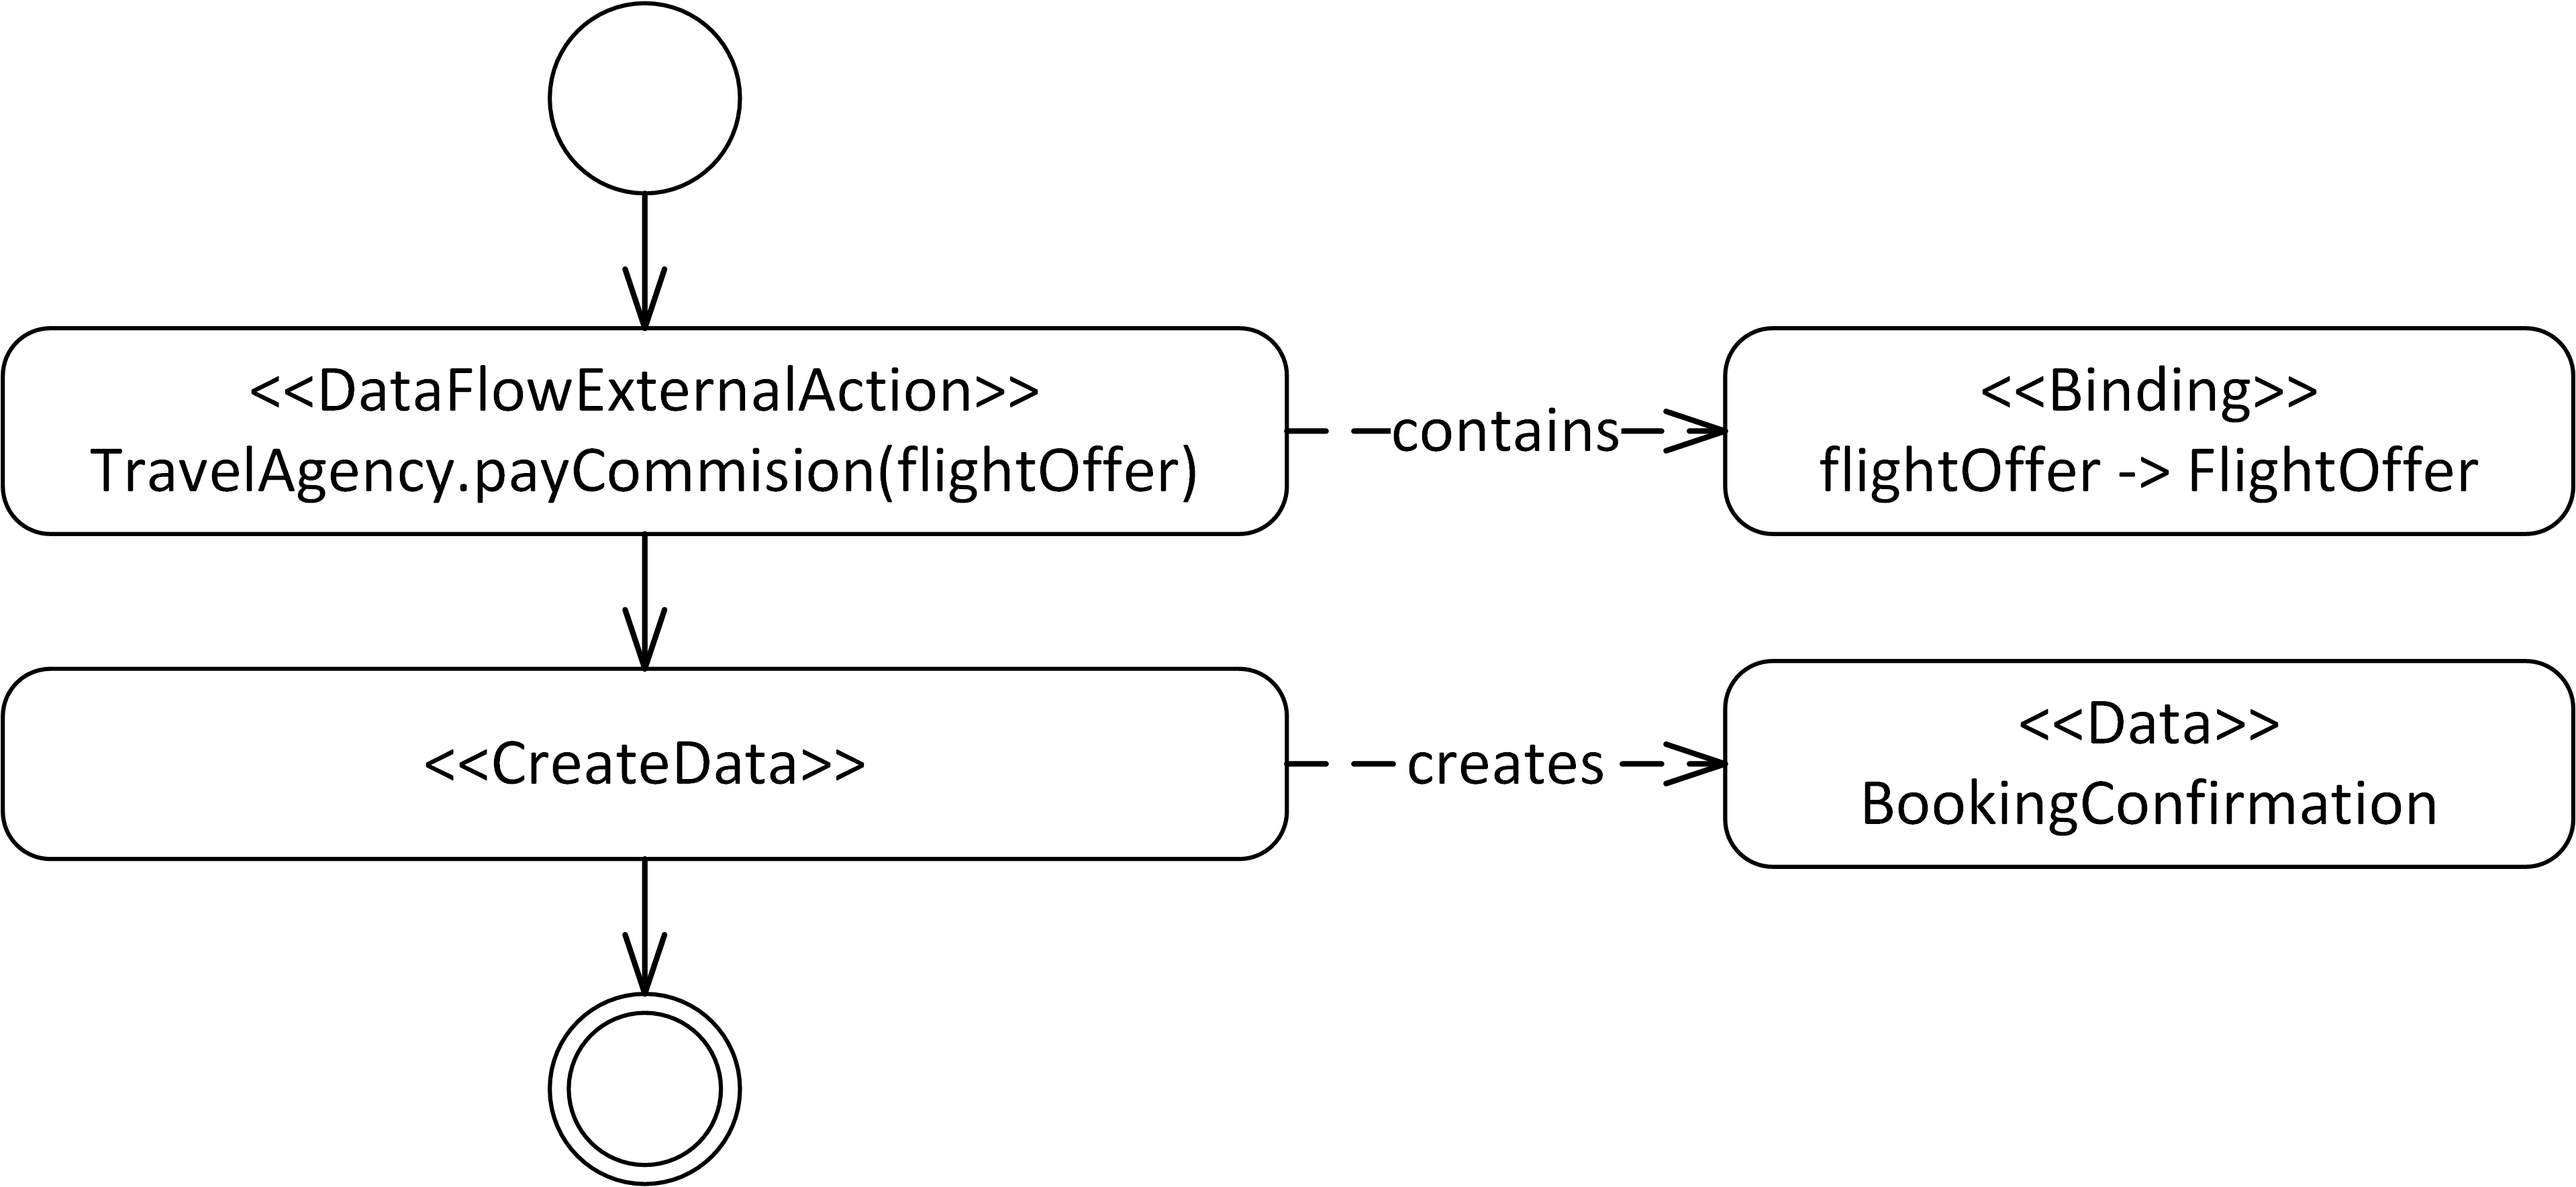
\includegraphics[width=0.7\textwidth]{images/dfseff_booking_bookFlight.png}
	\caption{DFSEFF des Aufrufs \texttt{Airline.bookFlight}}
	\label{img:df:booking:bookFlight}
\end{figure}

\subsection{Angreifermodell}
Vor der Vertraulichkeitsanalyse muss die Travelplanner-Modellinstanz, die mit Daten und Datenflüssen erweitert wurde, mit der Transformation aus \autoref{sec:implementierung} transformiert werden. Im Anschluss muss noch ein Angreifermodell erstellt werden. Da die Modellierung der Bachelorarbeit keinen Angreifer vorsieht, wird das Angreifermodell aus dem Vertraulichkeitsmodell (\autoref{sec:modellierung:confident}) wiederverwendet. Dieses Angreifermodell ist in \autoref{img:df:angreifer} abgebildet. Das abgebildete Angreifermodell setzt eine abgeschlossene Transformation und Datenflussanalyse voraus. In dem Angreifermodell gibt es drei Angreifer. Der Erste ist der Benutzer (\textit{User}). Dieser darf Zugang zu den Daten aus dem \texttt{DataSet} \textit{MobilePhone} haben. Außerdem hat der physikalischen Zugang zum Resource-Container \textit{MobilePhone} und zu den Linking-Resources \textit{4G+Internet} und \textit{OpenWifi+Internet}. Der Angreifer \textit{Airline}, darf nur auf Daten aus dem \texttt{DataSet} \textit{AirlineServer} zugreifen. Physikalischen Zugriff hat dieser nur auf den Resource-Container \textit{AirlineServer}. Der letzte Angreifer ist die \textit{TravelAgency}. Diese darf auf Daten aus dem \texttt{DataSet} \textit{AgencyServer} zugreifen und hat physikalischen Zugang zum Resource-Container \textit{AgencyServer}.

\begin{figure}[h]
	\centering
  	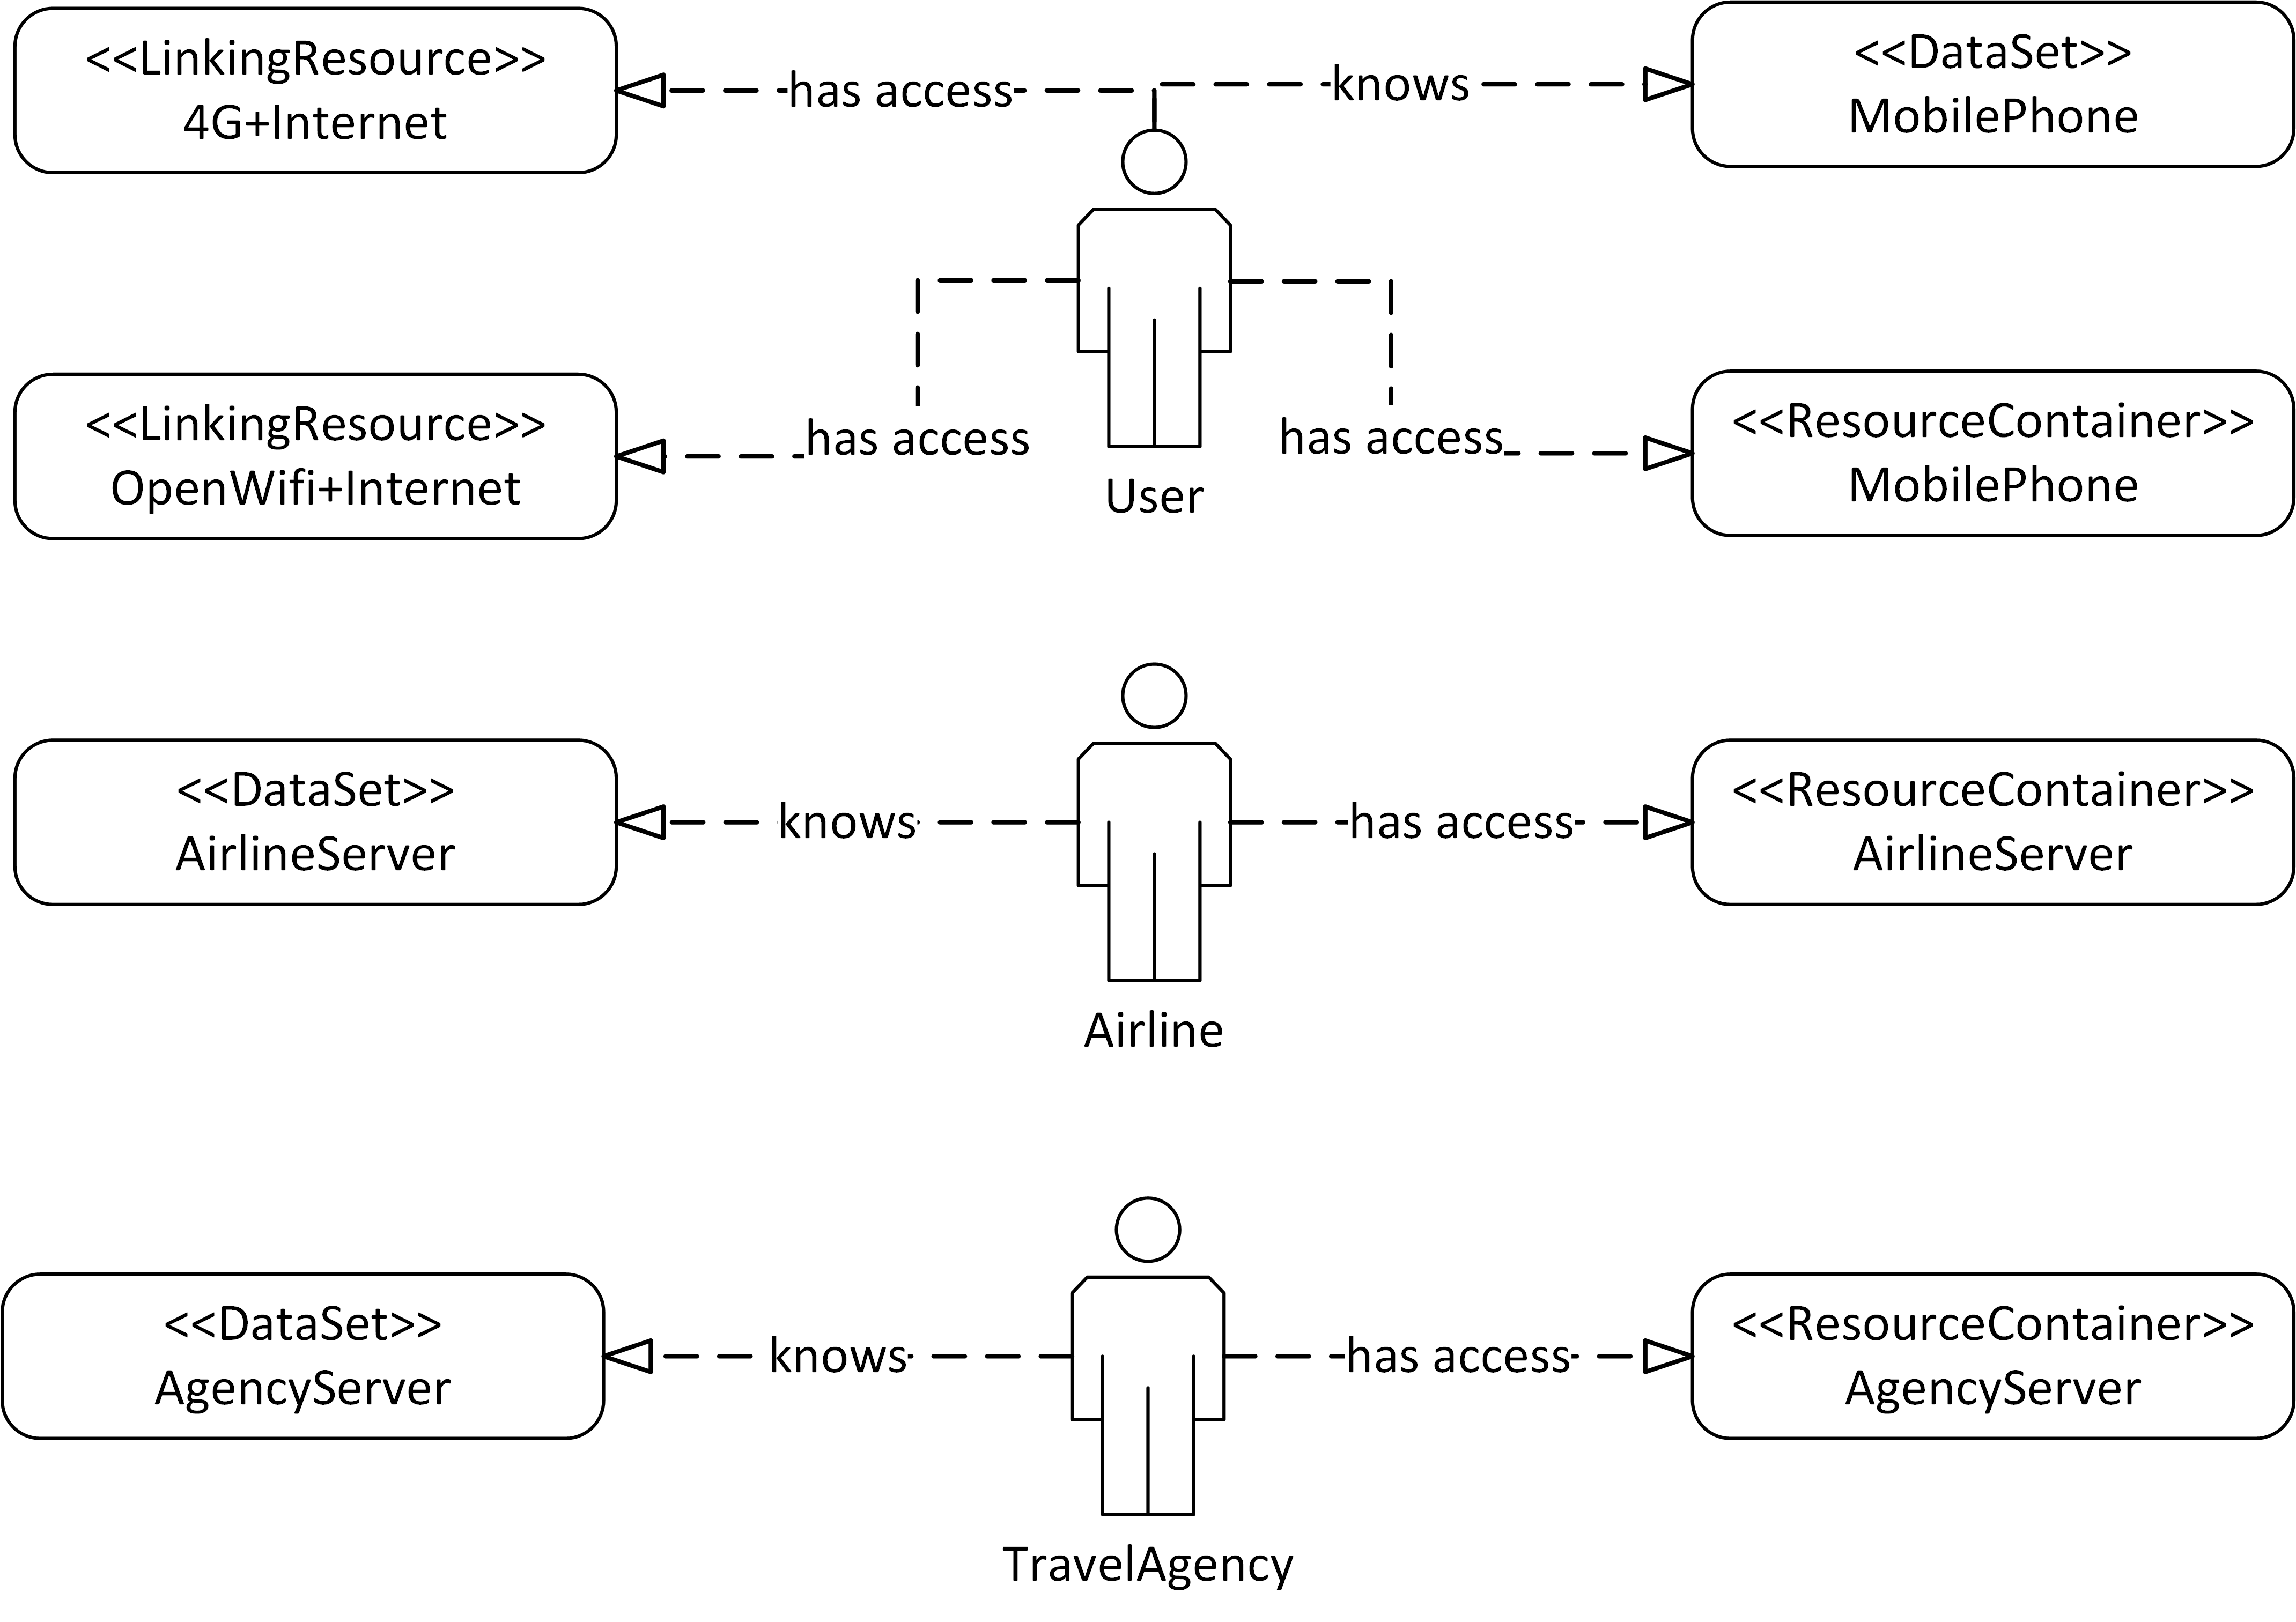
\includegraphics[width=0.9\textwidth]{images/travelplanner_angreifer.png}
	\caption{Angreifermodell der Modellinstanz, nachdem sie transformiert wurde}
	\label{img:df:angreifer}
\end{figure}

\section{Transformation und Datenflussanalyse}
\label{sec:implementierung}
Im Folgenden wird die Transformation beschrieben. Sie ist das letzte Ergebnis dieser Arbeit, nach dem Völter und Stahl Prozess. Es handelt sich um eine Transformation, die eine Modellinstanz aus \autoref{ch:modellierung} in eine Modellinstanz des Vertraulichkeitsmodells aus \autoref{sec:modellierung:confident} transformiert, um im Anschluss eine Vertraulichkeitsanalyse nach Kramer et. al. \cite{Kramera} durchführen zu können. \par
Die Transformation besteht aus einer \texttt{Generator}- und einer \texttt{Transformator}-Klasse. Der \texttt{Generator} ist für das Laden der Ressource und Modelle, sowie das Abspeichern des transformierten Modells zuständig. Der \texttt{Transformator} übernimmt die eigentliche Transformation. Die Transformation überträgt Elemente aus der Modellierung dieser Bachelorarbeit in Elemente des Vertraulichkeitsmodells. Außerdem werden die Datenflüsse analysiert. Nach der Analyse werden passende Elemente für das Vertraulichkeitsmodell erstellt. Im Folgenden soll diese Analyse und Transformation beschrieben werden. \par 
Die Datenflussanalyse verfolgt die Daten durch das System, die zuvor vom Benutzer eingegeben wurden. Dabei wird für jedes Datum, die durchlaufenden Komponenten gesammelt. Das Sammeln geschieht mithilfe der Klasse \texttt{BindingAndComponentPair}. Die Klasse besteht aus einem Feld für ein \texttt{Binding} und einem Feld für alle Komponenten, durch die dieses \texttt{Binding} geflossen ist. Ist der Datenfluss wieder beim Ursprung angelangt, werden die einzelnen Daten in \texttt{DataSet}s eingeordnet. Dabei wird für jeden Resource-Container aus dem Ressourcen-Umgebungs-Modell ein \texttt{DataSet} erstellt. Mithilfe des Komponenten-Allokations-Modells kann identifiziert werden, welche Komponente auf welchem Resource-Container ausgeführt wird. Daten die durch eine Komponente geflossen sind, werden in das \texttt{DataSet} eingeordnet, das zu dem Resource-Container gehört, auf dem die Komponente ausgeführt wird. Dabei wird aus einem Datum ein \texttt{Parameter-\\AndDataPair}. In das \texttt{ParameterAndDataPair} wird der Parameter aus dem \texttt{Binding} und alle \texttt{DataSet}s, durch die das Datum geflossen ist, eingetragen. \par
Zur Veranschaulichung der Transformation, soll \autoref{img:transformation:bsp} dienen. Die Abbildung stellt den Datenfluss des Aufrufs \texttt{BookingSelection.releaseCCD} als Datenflussdiagramm dar. Es wurde die Notation für Datenflussdiagramme aus \autoref{sec:datenflussdiagramm} verwendet. Zu Beginn identifiziert die Analyse, dass das Datum \textit{Airline} vom Benutzer aus, zur Komponente \texttt{Travelplanner} fließt. Daraufhin wird mithilfe eines neuen \texttt{BindingAndComponentPair} festgehalten, dass das \texttt{Binding}, des Datums, durch die \texttt{TravelPlanner} Komponente fließt. Im Anschluss fließt das Datum weiter zur \texttt{CreditCardCenter} Komponente. In das bestehende \texttt{BindingAndComponentPair} wird die \texttt{CreditCardCenter} Komponente hinzugefügt. Da der Datenfluss nicht weitergeht, wird das \texttt{BindingAndComponentPair} analysiert. Die Analyse kommt zu dem Schluss, dass das Datum \textit{Airline} durch die Komponenten \texttt{TravelPlanner} und \texttt{CreditCardCenter} geflossen ist. Daraufhin identifiziert sie, dass die beiden Komponenten auf dem selben Resource-Container ausgeführt werden. Diese Information wird aus dem Komponenten-Allokations-Modell abgeleitet (hier: \autoref{sec:appendix:travelplanner:system}). Daraufhin erstellt sie ein \texttt{DataSet} mit dem Namen des Resource-Containers. In diesem Fall wird ein \texttt{DataSet} mit dem Namen \textit{MobilePhone} erstellt. Da das Vertraulichkeitsmodell das Verhalten zwischen Parametern und nicht Daten betrachtet, wird der Parameter \textit{airline}, der mit dem Datum \textit{Airline} verknüpft ist identifiziert. Mithilfe eines \texttt{ParameterAndData-\\Pair} aus dem Vertraulichkeitsmodell, wird dieser Parameter mit dem \texttt{DataSet} \textit{MobilePhone} verknüpft. \par
\begin{figure}[h]
	\centering
  	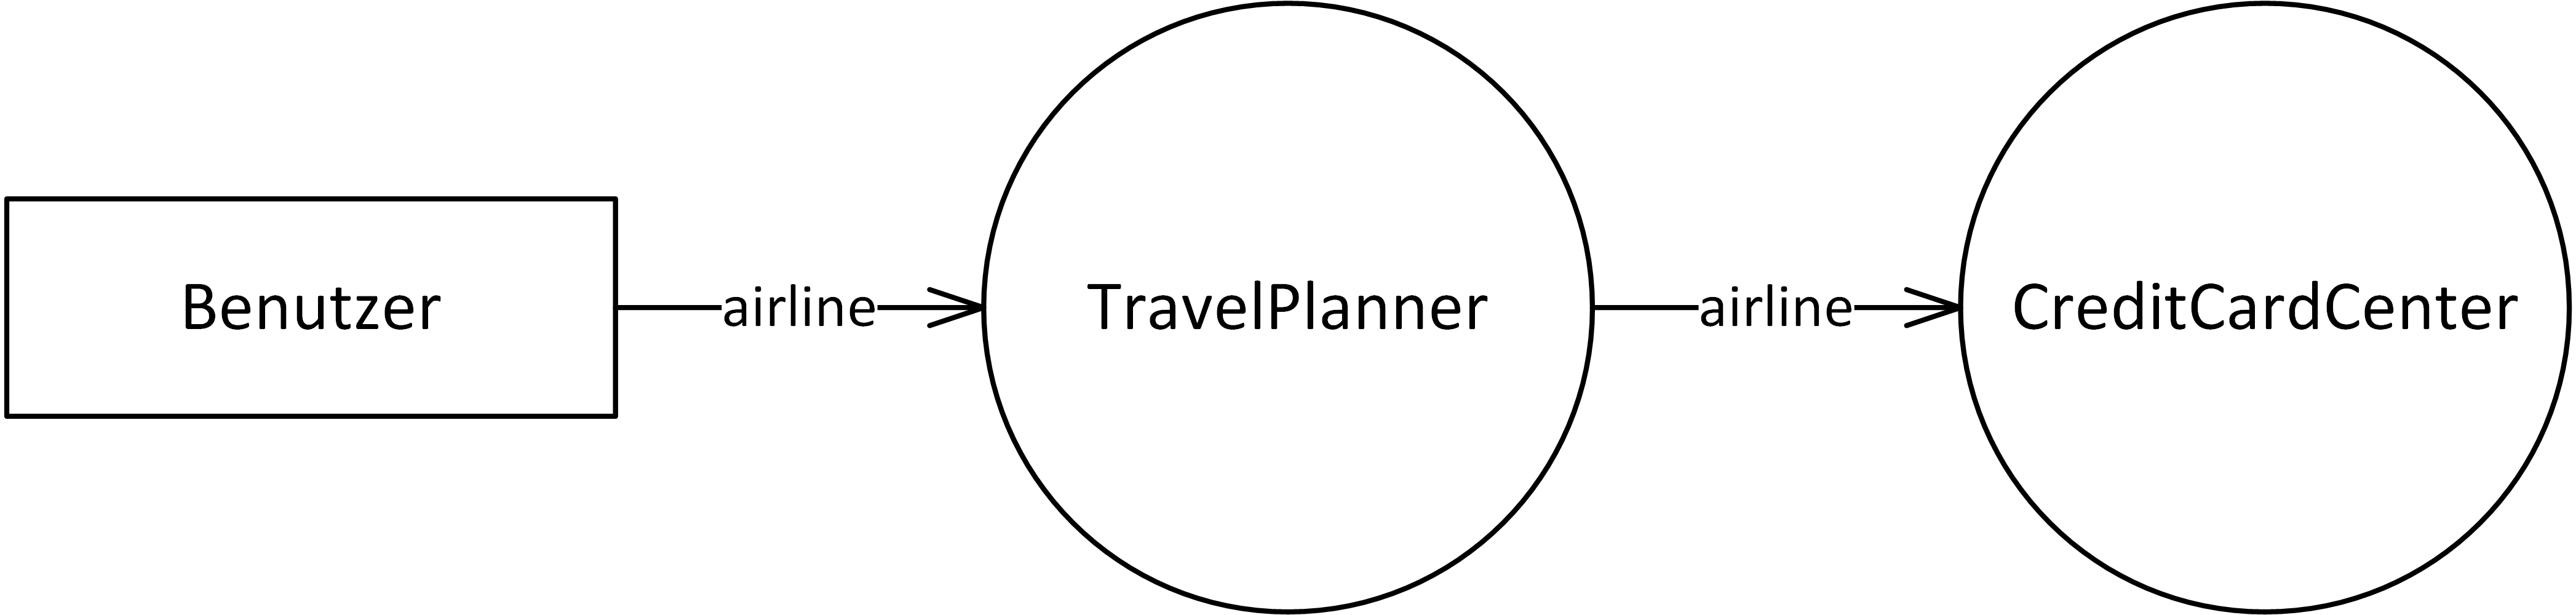
\includegraphics[width=0.9\textwidth]{images/transformation_bsp.png}
	\caption{Beispiel Datenfluss für die Transformation}
	\label{img:transformation:bsp}
\end{figure}

Elemente des Ressourcen-Umgebungs-Modells, aus \autoref{sec:stereotypes}, werden außerdem in ein vergleichbares Element aus dem Vertraulichkeitsmodell transformiert. Dabei werden aus \texttt{ResourceContainerPropertyContainer} und \texttt{LinkingResourcePropertyContainer} jeweils ein \texttt{LocationAndTamperProtectionPair}. Die \texttt{Location}-Elemente, die in den Containern enthalten sind, werden dabei auf \texttt{Location}-Elemente aus dem Vertraulichkeitsmodell abgebildet. Weitere Elemente aus der Erweiterung wurden nicht umgesetzt, da diese im Fallbeispiel nicht vorkommen.

%\section{Vertraulichkeitsanalyse}
%\label{sec:vertraulichkeitsanalyse}
%Diese Analyse prüft die Vertraulichkeit in komponentenbasierten Systemen. Für die Analyse müssen Eingabe und Ausgabe eines Systems spezifiziert werden, sowie Zugriffsspezifikation für Hardware und Kommunikationsverbindungen. Mithilfe dieser Informationen und einem Angreifer Modell wird eine Architektur- und Code-Analyse durchgeführt. Nach Durchführung der Analysewerden Designfehler, Datenlecks und Verstöße gegen die Spezifikation angezeigt. \\
%Für die Vertraulichkeitsanalyse müssen Eingabe und Ausgabe eines Systems spezifiziert werden, sowie Zugriffsspezifikation für Hardware und Kommunikationsverbindungen. Dazu müssen die Elemente aus dem Vertraulichkeitsmodell in das zu untersuchende System integriert werden. Dies ist mithilfe von MDSDProfiles möglich \cite{Kramer2012}. MDSDProfiles basieren auf EMF-Profiles und erlaubt es das Meta-Modell mit einem Profiles-Modell zu erweitern, ohne dieses ändern zu müssen. Das Profiles-Modell besteht dabei aus Stereotypen. Ein Stereotyp besteht aus einer Referenz zu einem Element, dass erweitert werden soll und aus einer Referenz zu dem Element, dass erweitern soll. Mithilfe dieser Stereotypes können Elemente durch Annotationen erweitert werden. \par
%Um die Ergebnisse aus der Transformation in das PCM Modell zu integrieren, benötigt es zwei der Stereotypen. Diese beiden sind in \autoref{img:profiles} abgebildet. Mithilfe des \texttt{InformationFlow}-Stereotypen lässt sich das Komponenten-Repository-Modell um einen Informationsfluss erweitern. Dabei können \texttt{ParameterAndDataPair}-Elemente an eine Signatur oder Schnittstelle im Komponenten-Repository-Modell angehängt werden. Der \texttt{LocationAndTamper}-Stereotype erweitert das Ressourcen-Umgebungs-Modell um eine Zugangsspezifikation. \texttt{LocatonAndTamperPair}-Elemente können somit Resource-Container und Linking-Resources im Ressourcen-Umgebungs-Modell erweitern. \par
%Diese beiden Modelle, das Profiles-Modell und die restlichen PCM-Modell dienen als Eingabe für die Vertraulichkeitsanalyse. \par
%Da eine Modellinstanz der Modellierung aus \autoref{ch:modellierung} durch die Analyse analysiert werden soll, muss diese zunächst transformiert werden. Im Anschluss muss die Transformation mithilfe der Stereotypes aus dem Profiles-Modell mit dem Komponenten-Repository-Modell und Ressourcen-Umgebungs-Modell verknüpft werden. Erst dann kann die Vertraulichkeitsanalyse angewendet werden.
%\begin{figure}[h]
%	\centering
 % 	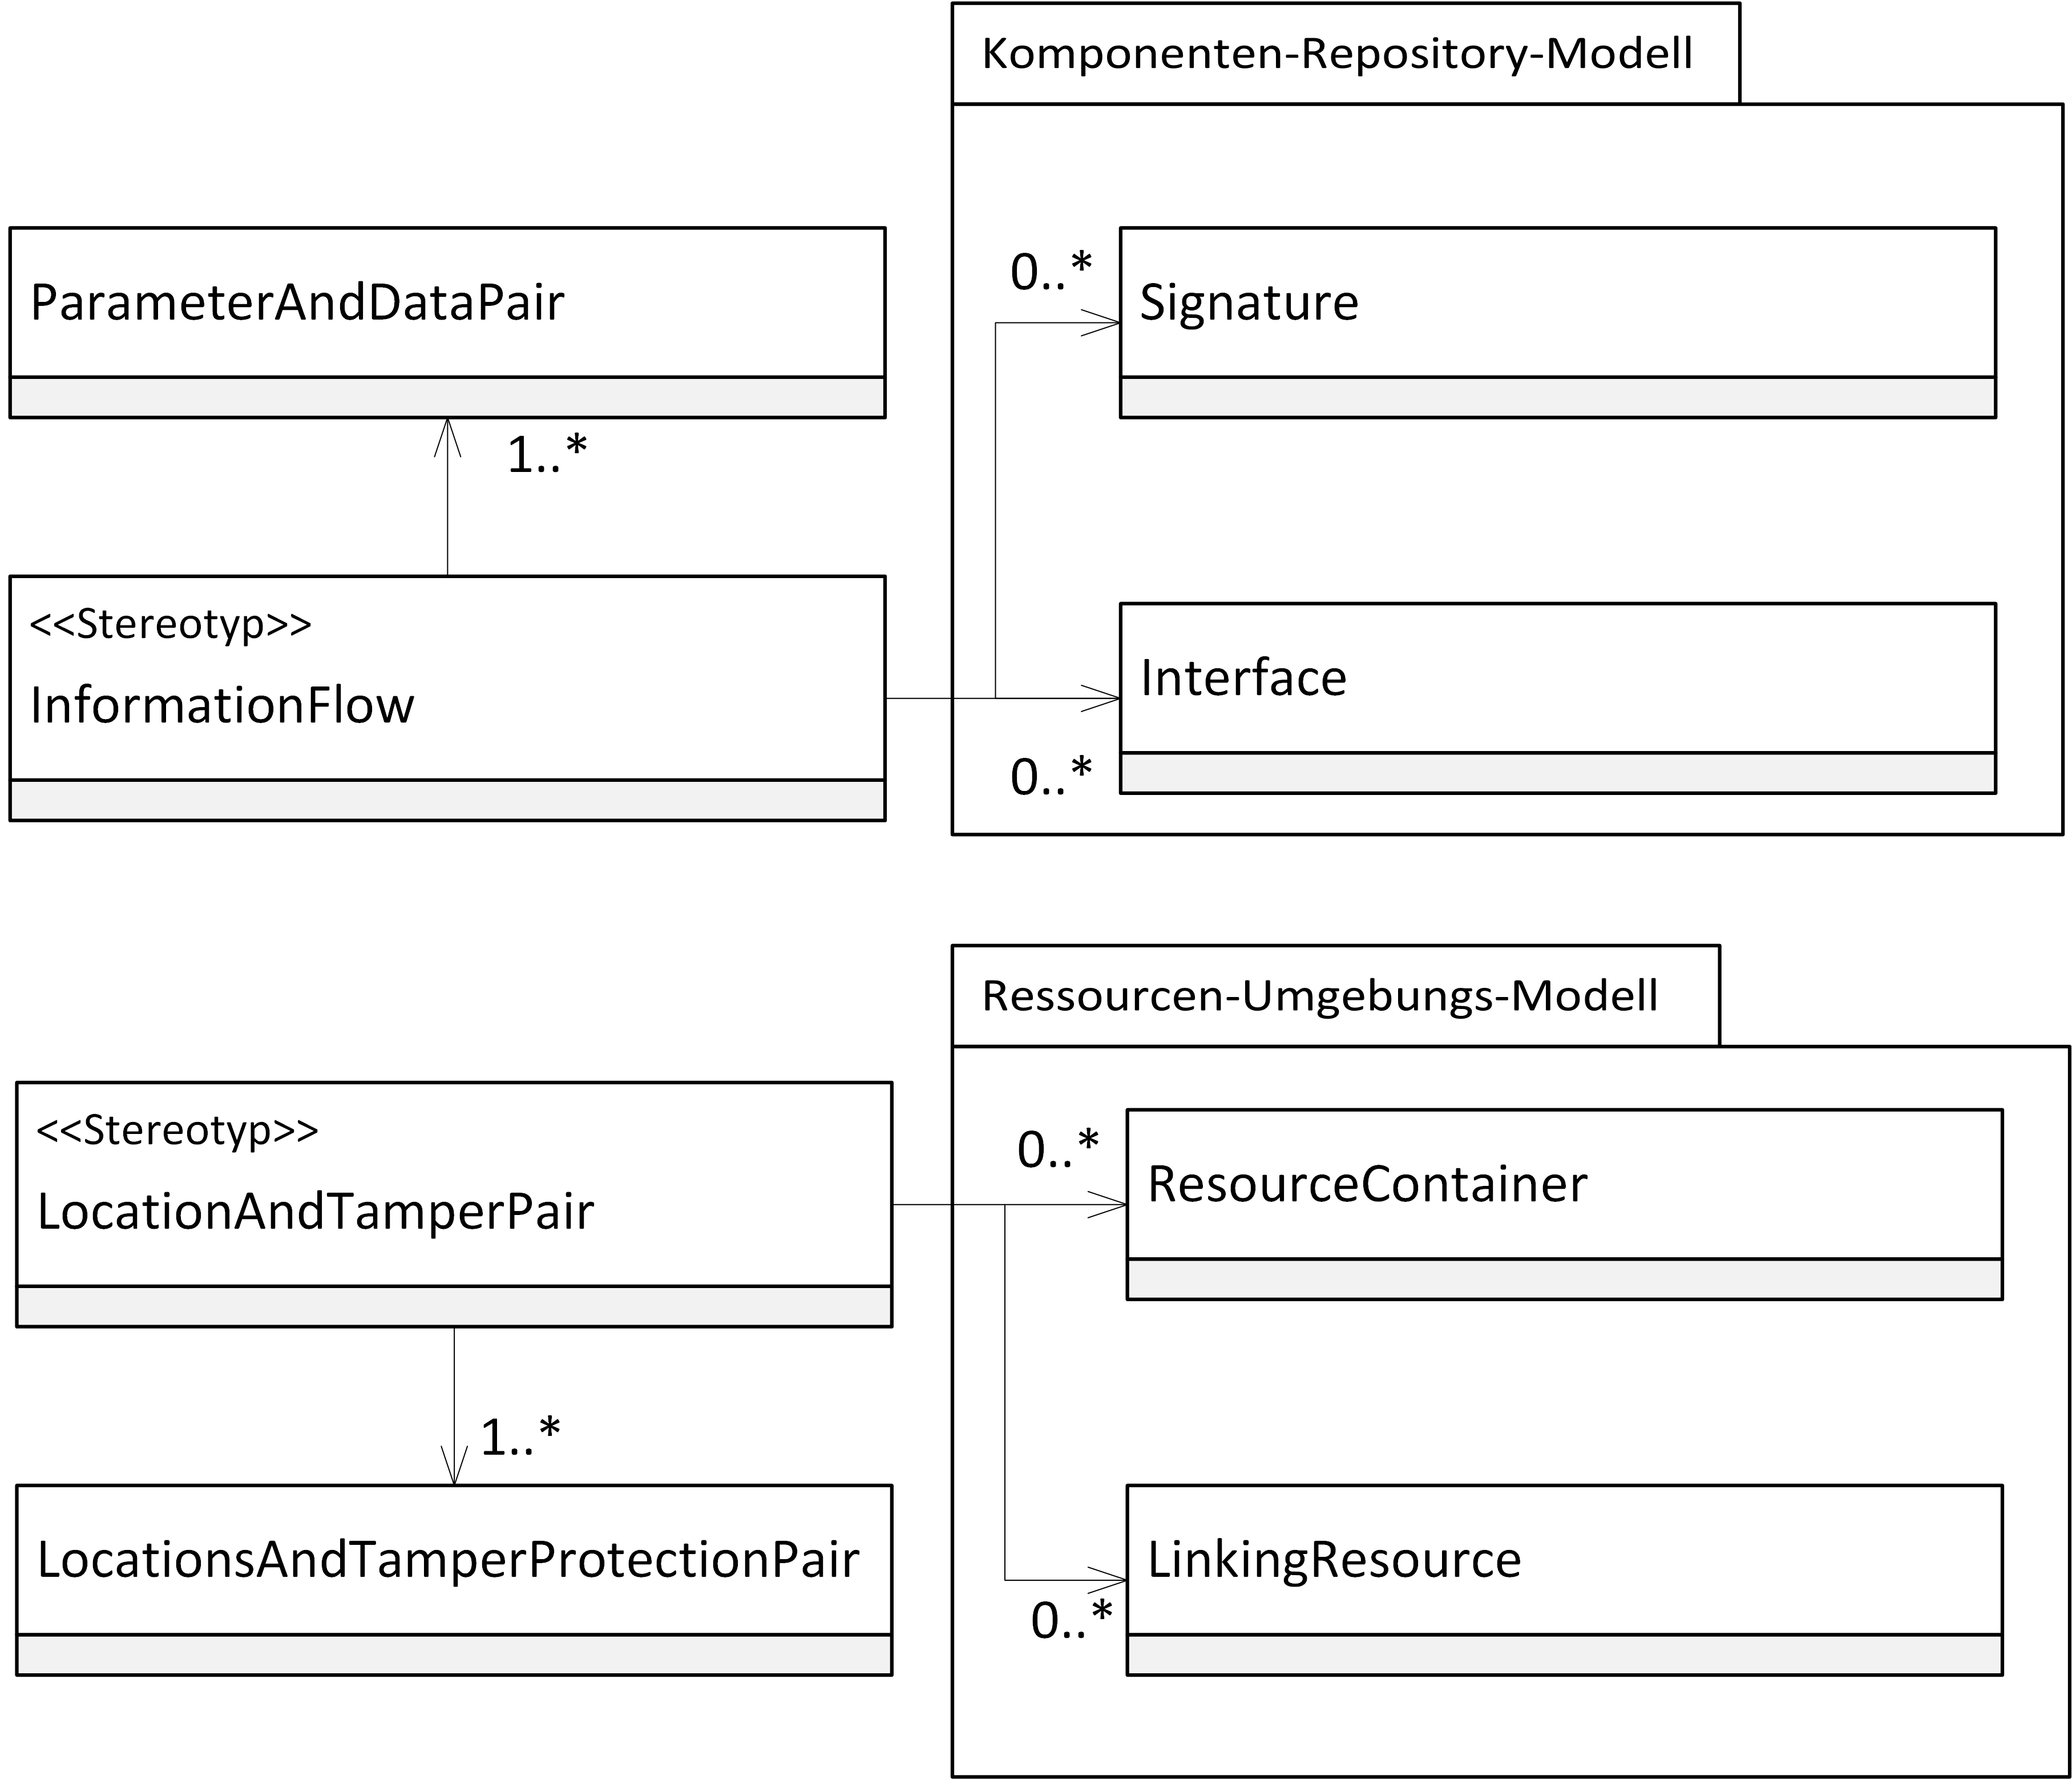
\includegraphics[width=0.7\textwidth]{images/profiles.png}
%	\caption{Stereotypen, mit denen das \gls{pcm} um Elemente aus dem Vertraulichkeitsmodell erweitert werden kann}
%	\label{img:profiles}
%\end{figure}

\section{Ergebnisse}
In diesem Abschnitt sollen die Ergebnisse der Validierung vorgestellt werden. Dazu werden die GQM-Fragen aus \autoref{tab:gqm} beantwortet. Die Antworten zu den Metriken können aus \autoref{tab:gqm:antworten} entnommen werden. 
\begin{table}[h]
\centering
\begin{tabular}{l|l}
\textbf{Metrik} & \textbf{Antwort} \\\hline
\textit{M1} & Alle Daten und Datenflüsse aus \autoref{img:travelplanner:seq:new} konnten \\
 & modelliert werden \\\hline
\textit{M2} & 0 Informationen müssen nochmal modelliert werden  \\\hline 
\textit{M3} & 78 neue Elemente mussten erstellt werden  \\ \hline 
\textit{M4} & Alle Daten konnten in \texttt{DataSet}s eingeordnet werden \\\hline
\textit{M5} & Ja, es ist ein valides Modell generiert worden  \\\hline 
\textit{M6} & Keine eindeutige Antwort, da Analyse nicht funktionsfähig  \\ \hline 
 
\end{tabular}
\caption{\label{tab:gqm:antworten} Antworten zu den Fragen aus \autoref{tab:gqm}}
\end{table}

Dazu wurde das Fallbeispiel aus \autoref{sec:travelplanner} um Daten und Datenflüsse erweitert. Dies wurde in \autoref{sec:travelplanner:modellierung} beschrieben. Die Daten und Datenflüsse wurden aus dem Sequenzdiagramm aus \autoref{img:travelplanner:seq:new} abgeleitet. Die identifizierten Datenflüsse konnten alle modelliert werden (M1). Bei der Modellierung konnten die Elemente, der PCM-Modelle aus \autoref{sec:travelplanner:pcm}, wiederverwendet werden und mussten nicht neu modelliert werden (M2). Bei der Modellierung der Daten und Datenflüsse mussten 78 neue Elemente erstellt werden (M3). Von diesen 78 Elementen wurden zwölf für die Hardware-Spezifikation im Ressourcen-Umgebungs-Modell erstellt. 45 Elemente haben die \gls{dfseff}s im Komponenten-Repository-Modell modelliert. Weitere 14 Elemente haben Datenflüsse im Nutzungsmodell modelliert und sechs Elemente haben Daten modelliert. Im Anschluss wurde das Datenflussmodell mit einer Datenflussanalyse analysiert und für die Vertraulichkeitsanalyse transformiert. Die Datenflussanalyse und Transformation wurde in \autoref{sec:implementierung} beschrieben. Dabei konnten alle modellierten Daten in \texttt{DataSet}s eingeordnet werden (M4). %Die Zuordnung ist in \autoref{tab:transformation:datasets} abgebildet. 
%\begin{table}
%\centering
%\begin{tabular}{l|c|c|c}
%\textbf{Binding} & \multicolumn{3}{l}{\textbf{DataSet}}\\\hline
%\textbf{(Data, Parameter)} & \textbf{MobilePhone} & \textbf{AirlineServer} & \textbf{AgencyServer} \\\hline
%\textit{(CCDecl, cc\_decl)} & x & x & \\\hline
%\textit{(CCD, ccd)} & x & & \\\hline
%\textit{(FlightBookedConfirmation, return)}  & x & x & x \\\hline
%\textit{(RequestData, reqestData)}  & x & x & x \\\hline
%\textit{(Airline, airline)}  & x & & \\\hline
%\textit{(FlightOffer, flightOffer)}  & x & x & x \\\hline
%\textit{(FlightOfferReturn, return)}  & x & x & x \\\hline 
%\end{tabular}
%\caption{\label{tab:transformation:datasets} Zuordnung von Daten zu %\texttt{DataSet}s nach der Datenflussanalyse aus \autoref{sec:implementierung}}
%\end{table}
Das transformierte Modell war valide (M5). Das Modell konnte in der Vertraulichkeitsanalyse verwendet werden (M6), konnte aber kein Ergebnis liefern. Der Grund, wieso die Analyse kein Ergebnis geliefert hat ist, dass die Vertraulichkeitsanalyse zum Validierungszeitpunkt defekt war. Das Travelplanner-Modell aus der Arbeit von Kramer et. al. \cite{Kramera} konnte auch nicht, mit der Vertraulichkeitsanalyse, analysiert werden. \par 
Da dieser Schritt nicht funktioniert, soll im Folgenden die Modellinstanz, aus der Arbeit von Kramer at. el. \cite{Kramera}, mit der transformierten Modellinstanz dieser Bachelorarbeit verglichen werden. Die beiden Modelle enthalten lediglich die Elemente \texttt{DataSet}, \texttt{Location}, \texttt{LocationAndTamperProtectionPair} und \texttt{ParameterAndDataPair}. Der erste Unterschied findet sich in den \texttt{DataSet}s. Das Vertraulichkeitsmodell enthält die \texttt{DataSet}s \textit{User}, \textit{Airline} und \textit{TravelAgency}. Das transformierte Modell enthält die \texttt{DataSet}s \textit{MobilePhone}, \textit{AgencyServer} und \textit{AirlineServer}. Dieser Unterschied kann jedoch vernachlässigt werden, da die \texttt{DataSet}s von der Bedeutung her, die Gleichen sind. Zum Vereinfachen der Beschreibung der Unterschiede werden die \texttt{DataSet}s, des transformierten Modells, auf die des Vertraulichkeitsmodells abgebildet. Somit entsteht die Zuordnung: \textit{MobilePhone} -> \textit{User}, \textit{AgencyServer} -> \textit{TravelAgency} und \textit{AirlineServer} -> \textit{Airline}. Die Hardware-Spezifikationen für das Ressourcen-Umgebungs-Modell sind in beiden Modellen gleich und werden im weiteren Verlauf der Bachelorarbeit nicht weiter betrachtet. Stattdessen werden die \texttt{ParameterAndDataPair}-Elemente der beiden Modelle verglichen. Dabei ist zu beachten, dass das Vertraulichkeitsmodell nicht an das neue Komponenten-Repository-Modell aus \autoref{sec:travelplanner:pcm} angepasst wurde. Die Unterschiede können aus \autoref{tab:data:unterschiede} entnommen werden. Der erste Unterschied findet sich in dem Dienst \texttt{Commision.pay-\\Commision}. Da dieser Dienst, wie in \autoref{sec:travelplanner:pcm} beschrieben, um einen Rückgabetyp und einen Parameter erweitert wurde, findet sich im Vertraulichkeitsmodell keine Zuordnung des Parameters und des Rückgabetyps (1, 2). Im transformierten Modell befindet sich der Parameter \textit{flightOffer} und der Rückgabewert in allen \texttt{DataSet}s. Der Grund hierfür ist, dass \textit{flightOffer} durch die Komponenten \textit{TravelPlanner}, \textit{Airline} und \textit{Travel-\\Agency} fließt. Diese Komponenten werden jeweils mit einem der \texttt{DataSet}s assoziiert, wie in der Transformation in \autoref{sec:implementierung} beschrieben. Der nächste Unterschied ist auch auf eine Änderung der Modellierung des Komponenten-Repository-Modells zurückzuführen. Der Dienst \texttt{BookingSelection.bookSelected} wurde um einen Parameter \textit{ccd\_decl} und um einen Rückgabewert erweitert. Dabei ist der Rückgabewert im transformierten Modell in allen \texttt{DataSet}s enthalten, da die Daten, bis zum Erstellen des Datums, durch alle Komponenten geflossen sind (5). Der Parameter \textit{cc\_decl} ist dabei nur in \textit{User} und \textit{Airline}, da dieser nicht an die \textit{TravelAgency}-Komponente weitergegeben wird (4). Der Parameter \textit{flightOffer} hingegen wird auch an die \textit{TravelAgency} weitergegeben und ist deshalb in allen drei \texttt{DataSet}s enthalten (3). Im Vertraulichkeitsmodell gibt es für \textit{cc\_decl} und den Rückagabewert keine Angaben. \textit{flightOffer} ist im Vertraulichkeitsmodell nur in \textit{User} und \textit{Airline} enthalten, da im alten Komponenten-Repository-Modell der Parameter nicht an die \textit{TravelAgency} über die Schnittstelle \textit{Commision} weitergegeben wird. D.h. nicht, dass die Analyse vorher falsch war, sondern, dass sich durch die genauere Modellierung der Architektur Änderungen ergeben haben. Bei dem Dienst \texttt{Booking.bookFlight} (10,11,12) sind die Gründe, für die Unterschiede, analog zu denen des Dienstes \texttt{BookingSelection.book-\\Selected} (3,4,5). Der Dienst \texttt{BookingSelection.getFlightOffers} wurde in der Bachelorarbeit um einen Rückgabewert erweitert. Deshalb kann das Vertraulichkeitsmodell hier keine Angabe zu den \texttt{DataSet}s machen (7). Bei dem Parameter \textit{requestData} gibt es in beiden Modellen keinen Unterschied (6). Dieser ist in allen \texttt{DataSet}s enthalten, da er durch die Komponenten \textit{Travelplaner}, \textit{TravelAgency} und \textit{Airline} fließt. Deshalb ist auch der Rückgabewert, im transformierten Modell, in allen \texttt{DataSet}s enthalten (7). Bei dem Dienst \texttt{FlightOffers.getFlightOffers} gibt es keinen Unterschied (8,9). Schließlich wurde auch der Dienst \texttt{Declassification.releaseCCD} um einen Rückgabewert erweitert. Das Vertraulichkeitsmodell bietet deshalb hier keine Angabe zu den \texttt{DataSet}s an (14). Bei dem Parameter \textit{airline} unterscheiden sich die beiden Modelle nicht (13). In beiden Modellen ist er im \texttt{DataSet} \textit{User} enthalten, da die Daten nur durch die CreditCardCenter Komponente fließen. Deshalb ist der Rückgabewert im transformierten Modell ebenfalls im \texttt{DataSet} \textit{User} enthalten. \par
Dieser Vergleich zeigt, dass die Unterschiede im transformierten Modell durchaus berechtigt sind und bei einer Anpassung des Modells, aus der Arbeit von Kramer et. al. \cite{Kramera}, zu den gleichen Ergebnissen führen sollten, sofern die Implementierung die Vertraulichkeit wahrt, sowie Implementierung und Spezifikation der Parameter-Data-Set-Zuordnung korrekt ist. \par 
Somit wurden die Ziele aus \autoref{tab:gqm} erreicht und eine Verhaltensspezifikation auf Datenflussebene in Palladio ermöglicht, die auch für Qualitätsvorhersagen, hier Vertraulichkeit, genutzt werden kann. \par
\begin{threeparttable}
\centering
\begin{tabular}{l|c|c|c|c|c|c}
\textbf{} & \multicolumn{3}{l}{\textbf{V-DS}} & \multicolumn{3}{|l}{\textbf{BA-DS}}\\\hline
\textbf{(Dienst, Parameter)} & \textbf{U} & \textbf{A} & \textbf{TA} & \textbf{U} & \textbf{A} & \textbf{TA} \\\hline
(1)\textit{(Commision.payCommision, flightOffer)} & k.A & k.A & k.A & x & x & x\\\hline
(2)\textit{(Commision.payCommision, return)} & k.A & k.A & k.A & x & x & x\\\hline
(3)\textit{(BookingSelection.bookSelected, flightOffer)} & x & x & & x & x & x\\\hline
(4)\textit{(BookingSelection.bookSelected, ccd\_decl)} & k.A & k.A & k.A & x & x & x\\\hline
(5)\textit{(BookingSelection.bookSelected, return)} & k.A & k.A & k.A & x & x & x\\\hline
(6)\textit{(BookingSelection.getFlightOffers, requestData)} & x & x & x & x & x & x\\\hline
(7)\textit{(BookingSelection.getFlightOffers, return)} & k.A & k.A & k.A & x & x & x\\\hline
(8)\textit{(FlightOffers.getFlightOffers, requestData)} & x & x & x & x & x & x\\\hline
(9)\textit{(FlightOffers.getFlightOffers, return)} & x & x & x & x & x & x\\\hline
(10)\textit{(Booking.bookFlight, fligthOffer)} & x & x & & x & x & x\\\hline
(11)\textit{(Booking.bookFlight, cc\_decl)} & k.A & k.A & k.A & x & x & \\\hline
(12)\textit{(Booking.bookFlight, return)} & x & x & x & x & x & x\\\hline
(13)\textit{(Declassification.releaseCCD, airline)} & x & & & x & & \\\hline
(14)\textit{(Declassification.releaseCCD, return)} & k.A & k.A & k.A & x & & \\\hline
\end{tabular}
\begin{tablenotes}
      \small
      \item V-DS: DataSet aus dem Vertraulichkeitsmodell, BA-DS: DataSet aus dem Modell der Bachelorarbeit, U: User, A: Airline, TA: TravelAgency
    \end{tablenotes}
\caption{\label{tab:data:unterschiede} Unterschiede der Zuordnung von Parameter in \texttt{DataSet}s}
\end{threeparttable}
% Die \texttt{LocationAndTamperProtextionPair}-Elemente sind ebenfalls identisch und  Obwohl der letzte Schritt der Validierung nicht funktioniert hat, konnte trotzdem ein valides Modell für die Vertraulichkeitsanalyse erstellt werden. Auch das Erweitern des Komponenten-Repository- und des Ressourcen-Umgebungs-Modells, durch die transformierten Elemente, mithilfe der MSDNProfiles war möglich und war valide. Deshalb kann davon ausgegangen werden, dass auch die Analyse ein valides Ergebnis geliefert hätte. \par

